% Exemplo de dissertação do INF-UFG com texto em portugues formatado com LaTeX
\documentclass[relatorio]{inf-ufg}
% Opções da classe inf-ufg (ao usar mais de uma, separe por vírgulas)
%   [tese]         -> Tese de doutorado.
%   [dissertacao]  -> Dissertação de mestrado (padrão).
%   [monografia]   -> Monografia de especialização.
%   [relatorio]    -> Relatório final de graduação.
%   [abnt]         -> Usa o estilo "abnt-alf" de citação bibliográfica.
%   [nocolorlinks] -> Os links de navegação no texto ficam na cor preta.
%                     Use esta opção para gerar o arquivo para impressão
%                     da versão final do seu texto!!!

% Fixar imagens com [H]
\usepackage{float}

%----------------------------------------------------- INICIO DO DOCUMENTO %
\begin{document}

%------------------------------------------ AUTOR, TÍTULO E DATA DE DEFESA %
\autor{Orlando da Cruz Pereira Júnior} % (José da Silva)
\autorR{da Cruz Pereira Júnior, Orlando} % (da Silva, José)

\titulo{Fatores habilitadores para definição de um modelo de negócio eletrônico}
\subtitulo{Um levantamento em empresas de pequeno e médio porte}

\cidade{Goiânia} % Nome da cidade em foi desenvolvido o trabalho
\dia{13} %
\mes{Dezembro} % Data da apresentação/defesa do trabalho
\ano{2019} % Formato numérico: \dia{01}, \mes{01} e \ano{2009}

%-------------------------------------------------------------- ORIENTADOR %
\orientador{Dr. Eliomar Araújo de Lima}
\orientadorR{Araújo de Lima, Eliomar}
% Use os comandos a seguir se for Orientadora e nao Orientador.
%\orientadora{\textless Nome da Orientadora\textgreater}
%\orientadoraR{\textless Nome Reverso da Orientadora\textgreater}

%\coorientador{\textless Nome do Co-orientador\textgreater}
%\coorientadorR{\textless Nome Reverso do Co-orientador\textgreater}
% Use os comandos a seguir se for Co-orientadora e nao Coorientador.
%\coorientadora{\textless Nome da Co-orientadora\textgreater}
%\coorientadoraR{\textless Nome Reverso da Co-orientadora\textgreater}

%-------------------------------------------------- INSTITUIÇÃO E PROGRAMA %
\universidade{Universidade Federal de Goiás} % {Universidade Federal de Goiás}
\uni{UFG}         % UFG
\unidade{Instituto de Informática} %Instituto de Informática
%\departamento{\textless Nome do Departamento\textgreater} %Unidades com mais de um depto.

%\universidadeco{\textless Nome da Universidade do Co-orientador\textgreater}
%\unico{\textless Sigla da Universidade do Co-orientador\textgreater}
%\unidadeco{\textless Nome da Unidade Acadêmica do Co-orientador\textgreater}

\programa{Computação} % Computação
\concentracao{Sistemas de Informação}

%-------------------------------------------------- ELEMENTOS PRÉ-TEXTUAIS %
\capa    % Gera o modelo da capa externa do trabalho
\publica % Gera a autorização para publicação em formato eletrônico
\rosto   % Primeira folha interna do trabalho

\begin{figure}[hbt!]
 \centering
  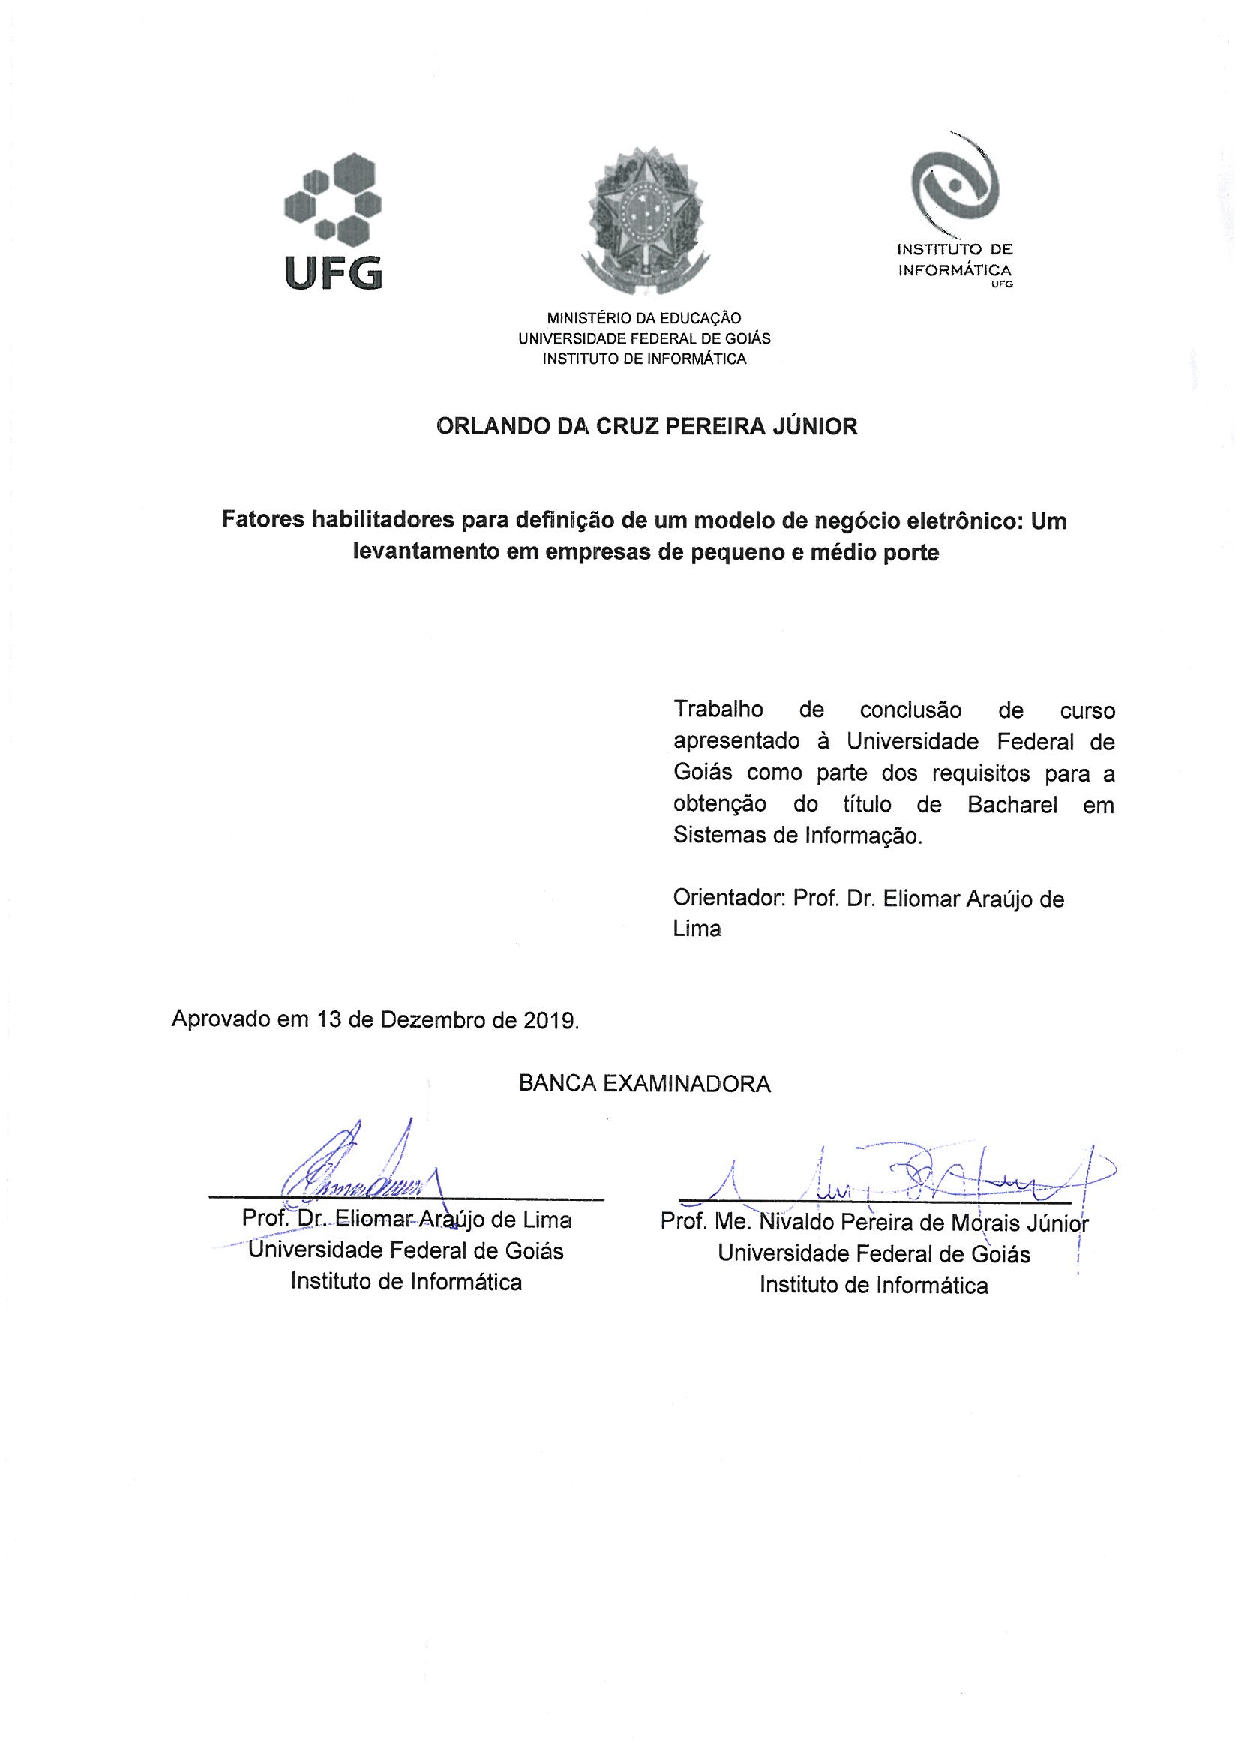
\includegraphics[width=\textwidth]{./aprov.pdf}
\end{figure}
\direitos{Graduando em Sistemas de Informação na UFG - Universidade Federal de Goiás. Sempre aplicou os conhecimentos obtidos na prática, buscando a inovação junto a comunidade acadêmica.}

\begin{dedicatoria}
Dedico este trabalho à meus familiares, em especial, meu pai e minha mãe.
\end{dedicatoria}

\begin{agradecimentos}

Em primeiro lugar agradeço a Deus pela oportunidade de estudar na Universidade Federal de Goiás. A fé em Deus me manteve motivado a continuar os estudos, mesmo diante das dificuldades.

Serei eternamente grato aos professores, pelas aulas ministradas sempre com excelência e sabedoria e aos meus amigos pela agradável companhia durante a graduação.

Ao professor Eliomar, meu orientador. Enquanto meu orientador, professor e mentor, me ensinou mais do que eu poderia escrever aqui. Ele vem me mostrado, por seu exemplo, como um bom profissional deve ser e agir. Sem sua ajuda e apoio do começo ao fim, este projeto não seria possível.

Por fim, agradeço a minha família, especialmente meus pais, que sempre me deram todo o apoio durante estes anos.

\end{agradecimentos}


\epigrafe{Muitos reclamam, "onde está a oportunidade?" A oportunidade está onde as queixas estão! Onde há problemas, há oportunidade!}
{Jack Ma - Fundador do grupo Alibaba}
{Em cerimôria da Organização das Nações Unidas - ONU. Nova York - EUA, 2014}

\chaves{e-business, empreendedorismo digital, posicionamento estratégico on-line para PME´s.}

\begin{resumo} 
Este trabalho tem como objetivo identificar os fatores habilitadores para definição de um modelo de negócio eletrônico para empresas de pequeno e médio porte. Pesquisas mostram que a grande maioria dos empreendimentos virtuais no Brasil são pequenas e médias empresas e que a maioria delas encerram suas atividades em um curto período de tempo. A importância da pesquisa torna-se evidente diante do aumento do número de empresas que estão ingressando neste mercado e do pouco conteúdo bibliográfico existente. A revisão bibliográfica identificou alguns fatores habilitadores, dentre eles, o conhecimento em tecnologia da informação; a terceirização; o uso dos marketplaces; gerenciamento de estoque com o método cross docking; atuação em um mercado de nicho; utilização de instrumento indicador (KPIs, KRIs), e por fim, a realização de análise ambiental, promovendo estudos de redesenho dos processos. Foi realizada uma pesquisa com o público alvo que revelou que as empresas com maior tempo de mercado possuem gestores com nível de conhecimento em tecnologia da informação “Bom” ou “Superior”, utilizam algum instrumento indicador (KPIs, KRIs) e fazem o acompanhamento durante o período de pós-venda, monitorando o feedback dos clientes na internet. Este trabalho contribui ao meio acadêmico pela abordagem utilizada, uma vez que a pesquisa buscou obter a visão dos proprietários das organizações, e com isso, permitindo o avanço do conhecimento na área.
\end{resumo}

\keys{e-business, digital entrepreneurship, online strategic positioning for SMEs.}

\begin{abstract}{Enabling factors for the definition of an electronic business model.}
This paper aims to identify the enabling factors for the definition of an electronic business model for small and medium sized companies. Research shows that the vast majority of virtual enterprises in Brazil are small and medium enterprises and most of them close down in a short period of time. The importance of research becomes evident given the increasing number of companies that are entering this market and the little existing bibliographic content. The literature review identified some enabling factors, including knowledge of information technology; outsourcing; the use of marketplaces; inventory management with the cross docking method; acting in a niche market; use of indicator instrument (KPIs, KRIs), and finally, the accomplishment of environmental analysis, promoting studies of process redesign. A survey was conducted with the target audience that revealed that companies with the longest market have managers with “Good” or “Higher” information technology knowledge, use some indicator tool (KPIs, KRIs) and follow up during the after-sales period by monitoring customer feedback on the internet. This work contributes to the academic environment by the approach used, since the research sought to obtain the vision of the owners of organizations, and thus, allowing the advance of knowledge in the area.
\end{abstract}


\tabelas[fig]
%Opções:
%nada [] -> Gera apenas o sumário
%fig     -> Gera o sumário e a lista de figuras
%tab     -> Sumário e lista de tabelas
%alg     -> Sumário e lista de algoritmos
%cod     -> Sumário e lista de códigos de programas
%
% Pode-se usar qualquer combinação dessas opções.
% Por exemplo:
%  figtab       -> Sumário e listas de figuras e tabelas
%  figtabcod    -> Sumário e listas de figuras, tabelas e
%                  códigos de programas
%  figtabalg    -> Sumário e listas de figuras, tabelas e algoritmos
%  figtabalgcod -> Sumário e listas de figuras, tabelas, algoritmos e
%                  códigos de programas

%--------------------------------------------------------------- CAPÍTULOS %

\chapter{Introdução}
\label{cap:intro}

O mercado brasileiro de e-commerce está em alta, mostrando que é uma oportunidade de negócio dinâmica e interessante, mas isso não quer dizer que seja simples manter um negócio online. Pesquisas mostram que as páginas dedicadas ao comércio eletrônico no país não costumam funcionar por muito tempo \cite{ecomnews} \cite{ecommerceschool2015}. Um levantamento feito pela empresa BigData Corp apurou que no ano de 2017 o tempo de vida dessas lojas foi em média, de 185 dias. Esse resultado foi obtido a partir da captura de dados em mais de 20 milhões de endereços brasileiros da internet \cite{sbvcsociedadebrasileiradevarejoeconsumo2017}.

A incapacidade de obter lucros é frequentemente vivenciada pelas organizações que trabalham com a internet no Brasil. No ano de 2013 por exemplo, a Dafiti, maior loja virtual de moda do Brasil, apresentava um prejuízo que representava cerca de 50\% o valor de seu faturamento. O número de varejistas on-line que crescem no Brasil, porém não lucram, é grande e traz nomes de organizações reconhecidas no mercado como Mobly, Casas Bahia, Ponto Frio, Netshoes \cite{rosanasantarosa2016}. 

Assim, podemos perceber que para muitas empresas a internet ainda não cumpriu suas promessas. Embora fazer negócio no ambiente digital possa ser original e estimulante, também pode ser frustrante, confuso e não lucrativo \cite{albertina.l.2010}. A B2W, grupo controlador das marcas Submarino, Americanas e Shoptime possue resultado que só vem decrescendo com o passar do tempo, deixando a mesma de operar com lucro em 2009 para adentrar em grandes prejuízos nos anos subsequentes, sendo que em 2011 o total de perdas alcançou o patamar negativo de R\$ 30 milhões, em 2012, de 42,83 milhões, e em 2013, de 10 milhões \cite{freitasc.2014}. Nestas grandes organizações o prejuizo pode estar de acordo com os planos traçados pelos gestores, com o objetivo de conquistar um lugar no mercado, o que não vem a ser o caso das PMEs.

Um estudo realizado sobre sobrevivência e mortalidade das empresas constatou que mercados que apresentam elevada taxa de entrantes são também aqueles com as maiores taxas de saída \cite{mourao2010}. Por volta do ano 2000 muitas empresas que atuavam na internet tinham modelos de negócios inviáveis baseados em expectativas oriundas do que era considerada a nova tecnologia \cite{motta2013}. Entre 2000-2001, em meio à explosão da bolha da internet, mais de 600 empresas on-line fecharam nos Estados Unidos e mais de 1.000 ao redor do mundo \cite{rosanasantarosa2016}. Essa quantidade de empresas pode parecer pequena, mais representa uma porcentagem significativa se comparada a quantidade de empresas que atuavam neste setor naquele momento. 

Apesar da crescente participação das empresas no comércio eletrónico, a grande maioria delas descobre que a simples presença na internet não se traduz em sucesso automático \cite{rosanasantarosa2016}. A pesquisa Profissionais de Ecommerce realizada pela Ecommerce School revelou que de uma base de aproximadamente 23 mil lojas virtuais no ar no Brasil, 70\% delas estavam abandonadas, ou seja, embora on-line não investiam em marketing para atrair visitantes e consequentemente não vendiam \cite{ecommerceschool2015}. 

Se um site não recebe visitas, os resultados são rapidamente sentidos pelos administradores do empreendimento virtual, podendo levar a uma decisão de renunciar aos esforços da empresa na internet \cite{rosanasantarosa2016}. Desta forma, ainda que novas formas de se conduzir os negócios tenham surgido, os fundamentos da competitividade empresarial se mantêm inalterados, seja para pequenos ou grandes empreendimentos \cite{porter2001}. 

As Pequenas e Médias Empresas PME’s enfrentam grandes obstáculos nesse ambiente, principalmente porque são caracterizadas por terem baixa intensidade de capital, poder decisório centralizado e a forte presença dos proprietários e familiares como mão-de-obra \cite{IBGE2003}. Esses empreendimentos não possuem uma definição específica. Existe uma variedade de critérios para essa classificação, ora pela legislação específica que leva em conta o faturamento da empresa, ora pelo Sebrae que leva em conta o número de pessoas ocupadas.

Alguns estudos relatam que fatores habilitadores para definição de um modelo de negócio eletrônico como estratégias a serem empregadas para o sucesso \cite{criticalfactors2012}. Esses fatores englobam um grupo restrito de áreas da empresa, de práticas ou de cargos ocupados considerados como chave para o sucesso de uma organização \cite{criticalfactors2014}. Desta forma, a definição da lógica de captura, entrega e proposição de valor de um negócio eletrônico pode impactar no índice de mortalidade dos negócios eletrônicos?

\section{Objetivos}
\label{subsec:framing}
%% - - - - - - - - - - - - - - - - - - - - - - - - - - - - - - - - - - --

Nesse contexto, o objetivo deste estudo é identificar quais são os fatores habilitadores candidatos para definição de um modelo de negócio eletrônico para empreendimentos de pequeno e médio porte que atuam no segmento de tecnologia da informação.

\section{Objetivos Específicos}
\label{subsec:framing}
%% - - - - - - - - - - - - - - - - - - - - - - - - - - - - - - - - - - -

Para alcançar o objetivo geral, os seguintes objetivos específicos foram definidos:

\begin{enumerate}
\item Identificar as causas que afetam o tempo de vida útil das PME´s no cenário eletrônico.
\item Descrever as características dos negócios digitais e os motivos que conduzem à sua ascensão.
\item Apresentar os princípios e abordagens do Modelo de Negócio - Canvas. 
\item Discorrer sobre os fatores internos e externos que exercem influência nas organizações.
\item Analisar e discutir os elementos contextuais que conduzem aos fatores habilitadores para definição de um modelo de negócio eletrônico.
\end{enumerate}

A estrutura e a organização deste trabalho foram delineadas da seguinte forma: o Capítulo \ref{cap:theory} apresenta a revisão da literatura, descrevendo o modelo de negócio, as características das pequenas e médias empresas e os fatores internos e externos que podem influenciar no seu sucesso; o Capítulo \ref{cap:texto} descreve a metodologia, mostrando como foi a trajetória da pesquisa até chegar ao resultado final; o Capítulo \ref{cap:results} apresenta os resultados obtidos  e o Capítulo \ref{cap:conclusion} apresenta a conclusão sobre este trabalho.






\chapter{Revisão da Literatura}
\label{cap:theory}

%% - - - - - - - - - - - - - - - - - - - - - - - - - - - - - - - - - - -
\section{Caracterização dos empreendimentos de pequeno e médio porte}
\label{sec:temp}

Internacionalmente não existe uma definição que delimite o conceito de PME devido a diferenças entre os países, sua economia e quantidade de empresas. No entanto, para fins de políticas públicas a União Europeia estabeleceu alguns critérios para definição das PME’s que leva em conta a dimensão da empresa em termos de pessoas ocupadas, faturamento, balanço e a estrutura de propriedade da empresa \cite{mpme2018}.

No Brasil observa-se também uma variedade de critérios para essa definição, tanto por parte da legislação específica, instituições financeiras oficiais e órgãos representativos do setor, que podem se basear pelo valor do faturamento da empresa, pelo número de pessoas ocupadas ou em ambos \cite{mpme2017}. Neste trabalho nos restringimos a analisar apenas dois deles:  o critério utilizado pela Receita Federal para a admissão ao regime tributário do Simples Nacional aplicável às microempresas (MEs) e empresas de pequeno porte (EPPs) e o de pessoal ocupado utilizado pelo Serviço Brasileiro de Apoio às Micro e Pequenas Empresas (Sebrae).

A definição que está na Lei Geral para Micro e Pequenas Empresas é a mais comum e é utilizada pela Receita Federal. De acordo com essa definição as microempresas são as que possuem um faturamento anual de, no máximo, R\$360 mil por ano. As pequenas devem faturar entre R\$360.000,01 e R\$3,6 milhões anualmente para ser enquadradas \cite{sebrae2016}.

O Sebrae em algumas de suas publicações utiliza como critério para definição das micro, pequenas e médias empresas o porte deste segmento empresarial em termos de pessoal ocupado. Segundo este critério de classificação, as micro empresas serão aquelas com até nove pessoas ocupadas nas atividades de serviço e comércio, e como pequenas empresas as que têm entre 10 e 49 pessoas ocupadas. Serão consideradas médias empresas as que possuírem de 50 a 99 pessoas ocupadas, como mostrado na tabela \ref{tab:classif} \cite{sebrae2013}.

% Please add the following required packages to your document preamble:
% \usepackage{multirow}
\begin{table}[]

{\renewcommand\arraystretch{1.25}}
 \caption{Classificação do porte de empresas no Brasil \cite{sebrae2013}.}
 \label{tab:classif}

\begin{tabular}{l|c|c|c|}
\cline{2-4}
\multirow{}{}{} & \begin{tabular}[c]{@{}c@{}}Legislação\\ brasileira\end{tabular} & \multicolumn{2}{c|}{SEBRAE} \\ \cline{2-4} 
 & \multirow{}{}{\begin{tabular}[c]{@{}c@{}}Faturamento bruto \\ anual\end{tabular}} & \multicolumn{2}{c|}{Número de funcionários} \\ \cline{3-4} 
 &  & Indústria & Comércio e serviços \\ \hline
\multicolumn{1}{|l|}{\begin{tabular}[c]{@{}l@{}}Empreendedor \\ individual\end{tabular}} & Até R\$81 mil & - & - \\ \hline
\multicolumn{1}{|l|}{Microempresa} & <R\$ 360 mil & até 19 & até 9 \\ \hline
\multicolumn{1}{|l|}{Pequena empresa} & \begin{tabular}[c]{@{}c@{}}\textgreater R\$ 360 mil\\ \\ <R\$ 3,6 milhões\end{tabular} & de 20 a 99 & de 10 a 49 \\ \hline
\multicolumn{1}{|l|}{Média empresa} & \begin{tabular}[c]{@{}c@{}}\textgreater R\$ 90 milhões\\ \\ <R\$ 300 milhões\end{tabular} & de 100 a 499 & de 50 a 99 \\ \hline
\multicolumn{1}{|l|}{Grande empresa} & >R\$ 300 milhões & 500 ou mais & 100 ou mais \\ \hline
\end{tabular}
\end{table}

%\subsection{Sub seção}
%\label{subsec:framing}
%% - - - - - - - - - - - - - - - - - - - - - - - - - - - - - - - - - - -
\section{Tempo de vida útil dos empreendimentos de pequeno e médio porte}
\label{sec:vidautil}

Pesquisas do Sebrae mostram que a falta de planejamento, deficiências na gestão e o próprio comportamento do empreendedor são as principais causas do fechamento de empresas em seus primeiros anos de atividade. Segundo a pesquisa cerca de 39\% ignoravam qual seria o capital de giro necessário para abrir a empresa, 38\% não sabia quantos concorrentes teria e 46\% afirmam ter iniciado o negócio sem conhecer os hábitos de consumo dos clientes nem o número de clientes que teriam \cite{sebraesp}.  

Pelo levantamento do Sebrae 55\% dos empresários não definiram um plano de negócios antes da abertura \cite{sebraesp}, documento que contém todos os detalhes do empreendimento como aspectos financeiros, mão de obra, estratégias de marketing, perfil do público-alvo, pontos fortes e fracos, riscos, oportunidades, em resumo, tudo o que o empreendedor tem de analisar para exercer sua atividade com mais segurança.

Se comparado com estabelecimentos físicos, o e-commerce por exemplo pode ser muito tentador, pois as barreiras de entrada são pequenas e em pouco tempo é possível montar uma e-loja e começar a trabalhar, desta forma muitas pessoas resolvem se aventurar. Neste caso o desafio para o empreendedor não está em abrir, mais sim em manter o negócio ativo no longo prazo \cite{ecomnews}. 

A facilidade de entrada deve-se a questões financeiras como a existência de muitas plataformas de e-commerce, que não exigem pagamento algum para que o negócio seja iniciado e também a integração destas lojas on line com meios de pagamento sem precisar pagar qualquer valor \cite{newtrade2017}.
 
Em levantamento feito em 2017, o Brasil possuía 590 mil lojas online, 31\% a mais que em 2015. No entanto, elas possuem um tempo de vida efêmera, cerca de 185 dias \cite{sbvcsociedadebrasileiradevarejoeconsumo2017}. Na tabela \ref{tab:fracasso} podemos ver algumas das causas do fracasso destas empresas. Um e-commerce recebe status de inativo quando para de ser acessado, atualizado ou receber qualquer tipo de interação por um período superior a 1 mês \cite{ecomnews}. 

% ######## init table ########
\begin{table}[h]
 \centering
% distancia entre a linha e o texto
 {\renewcommand\arraystretch{1.25}
 
  \caption{Resumo dos fatores associados ao fracasso do comércio eletrônico \cite{rosanasantarosa2016}. }
 \label{tab:fracasso}
 
 \begin{tabular}{ l }
  \cline{1-1}  
    \multicolumn{1}{|c|}{\textbf{FRACASSO} \centering }
  \\  
  \cline{1-1}  
    \multicolumn{1}{|c|}{Gestão do comércio eletrônico apenas como mais um canal \centering }
  \\  
  \cline{1-1}  
    \multicolumn{1}{|c|}{Expectativas irreais \centering }
  \\  
  \cline{1-1}  
    \multicolumn{1}{|c|}{Consideração equivocada de investimentos iniciais \centering }
  \\  
  \cline{1-1}  
    \multicolumn{1}{|c|}{Falta de investimentos em busca de visibilidade \centering }
  \\  
  \cline{1-1}  
    \multicolumn{1}{|c|}{Gestão especulativa \centering }
  \\  
  \cline{1-1}  
    \multicolumn{1}{|c|}{Falta de domínio das estratégias de negócios e TI \centering }
  \\  
  \cline{1-1}  
    \multicolumn{1}{|c|}{Falta de políticas de cooperação \centering }
  \\  
  \cline{1-1}  
    \multicolumn{1}{|c|}{Uso de tecnologia incapaz de suportar as vendas \centering }
  \\  
  \cline{1-1}  
    \multicolumn{1}{|c|}{Logística de entrega inadequada \centering }
  \\  
  \hline

 \end{tabular} }
\end{table}

As empresas que atuam de forma física enfrentam alguns fatores associados ao fracasso similares as empresas que atuam de forma eletrônica. Estas empresas físicas também possuem os causadores do fracasso específicos desta área, como por exemplo errar na escolha do local adequado para o novo negócio, não saber vender ou promover os produtos/serviços e não saber tratar adequadamente o cliente \cite{idalbertochiavenato2007}. Na tabela \ref{tab:fracassofisica} podemos ver os principais fatores associados ao fracasso das empresas que atuam de forma física.

% ######## init table ########
\begin{table}[H]
 \centering
% distancia entre a linha e o texto
 {\renewcommand\arraystretch{1.25}
 
  \caption{Resumo dos fatores associados ao fracasso das empresas que atuam de forma física. \cite{idalbertochiavenato2007}. }
 \label{tab:fracassofisica}
 
 \begin{tabular}{ l }
  \cline{1-1}  
    \multicolumn{1}{|c|}{\textbf{FRACASSO} \centering }
  \\  
  \cline{1-1}  
    \multicolumn{1}{|c|}{Incompetência do empreendedor \centering }
  \\  
  \cline{1-1}  
    \multicolumn{1}{|c|}{Falta de experiência de campo \centering }
  \\  
  \cline{1-1}  
    \multicolumn{1}{|c|}{Mercado consumidor restrito \centering }
  \\  
  \cline{1-1}  
    \multicolumn{1}{|c|}{Comportamento do empreendedor \centering }
  \\  
  \cline{1-1}  
    \multicolumn{1}{|c|}{Localização inadequada \centering }
  \\  
  \cline{1-1}  
    \multicolumn{1}{|c|}{Despesas operacionais elevadas \centering }
  \\  
  \cline{1-1}  
    \multicolumn{1}{|c|}{Dificuldade de estoque \centering }
  \\  
  \hline

 \end{tabular} }
\end{table}

A conversão média de compras no Brasil em lojas virtuais é de 1.6\% das visitas, o que significa que, a cada 1000 visitas, 16 convertem em venda \cite{sebrae2019}. Segundo a pequisa feita pelo Ebit, cerca de 27,3\% das compras em 2017 foram efetuadas em tablets ou smartphones, reforçando a expansão desses canais na preferência dos consumidores \cite{ecombrasil2018}.

Segundo o Sebrae \cite{sebraesp}, o principal motivo para o empresário ter fechado o negócio é a falta de capital e obtenção de lucro. Ao fechar a empresa o empreendedor está encerrando um sonho, o desejo de ter o próprio negócio, o que gera sentimentos negativos no empreendedor, como tristeza, mágoa e frustração. Ainda há a perda financeira, onde mais da metade dos empresários perde tudo ou parte do dinheiro investido, dinheiro que na sua maior parte é próprio ou de familiares. Na figura \ref{fig:fracasso} podemos ver quanto um empresário perdeu em média com o encerramento do negócio, neste caso não considerando apenas os empreendimentos que atuam de forma eletrônica e sim as empresas no geral.

\begin{figure}[H]
 \centering
  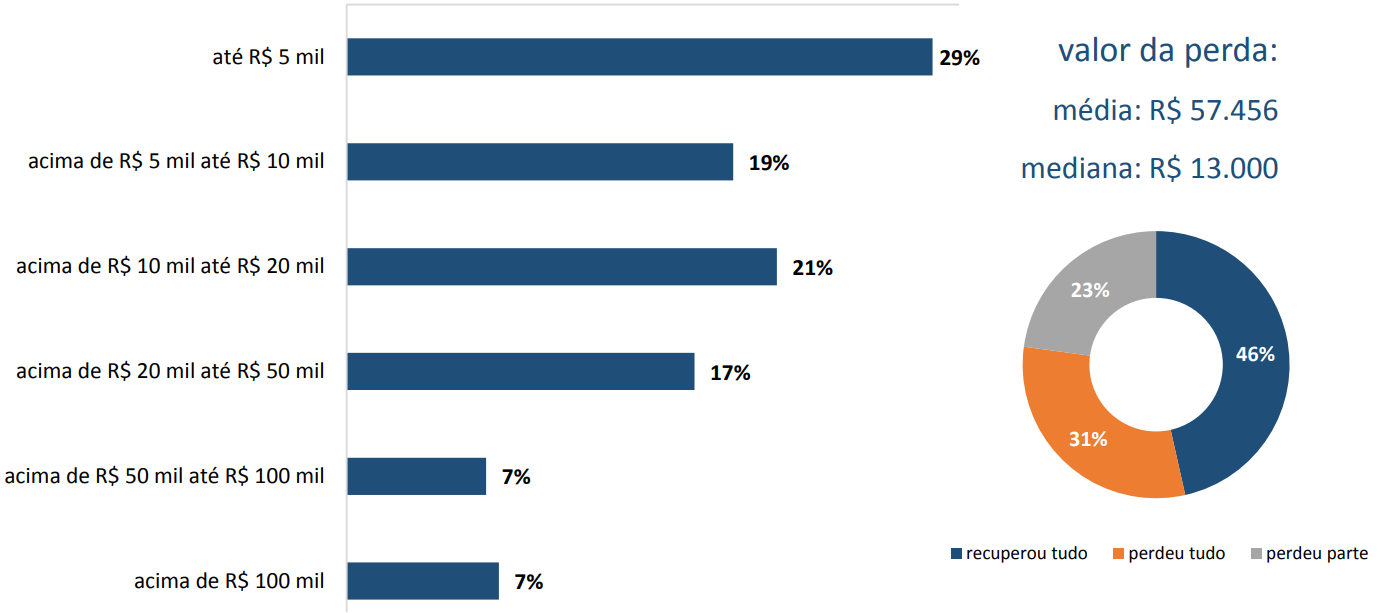
\includegraphics[width=0.80\textwidth]{./fig/valordoprejuizo}
 \caption{Quanto um empresário perdeu em média com o encerramento de sua empresa \cite{sebraesp}.}
 \label{fig:fracasso}
\end{figure}

%% - - - - - - - - - - - - - - - - - - - - - - - - - - - - - - - - - - -
\section{Negócios digitais e suas particularidades}
\label{sec:carac}

Com o passar do tempo o mundo está ficando cada vez mais digital, isso é representado pelo número crescente de pessoas que estão consumindo produtos e serviços pela internet. Com isto, pessoas, programas de computador e máquinas também precisam de dados sendo entregues com velocidade nunca vistos antes, o que exige novas práticas das empresas. Isso implica que estas empresas não somente cheguem a todos os lugares e integrem-se a tudo, mas que façam isso de modo direto, mais rápido e com segurança. É a Era da Interconectividade \cite{negdig2019}.

Esta nova Era permite que as empresas falem diretamente com qualquer integrante de sua cadeia de valor. Todos os setores envolvidos precisam de mais segurança em suas transações, como também de mais velocidade. Com a Interconexão as empresas ganham milissegundos essenciais na hora de vender um serviço ou produto e de entregá-los. A necessidade de entrar nessa nova Era é tão importante para as empresas que a velocidade da Interconexão deve quintuplicar globalmente nos próximos anos, chegando a mais de 8.200 terabits por segundo (Tbps) nos próximos dois anos. Velocidade de Interconexão é caracterizada como a capacidade total provisionada para a troca de tráfego, privada e direta, com um conjunto diverso de contrapartes e provedores, em pontos de troca de tráfego e TI distribuídos \cite{negdig2019}.

Os negócios digitais são caracterizados por fazerem uso da tecnologia e da internet para desenvolver e comercializar padrões mais modernos de produtos e serviços. É um novo conceito de mercado, revolucionado pela web, em que consumidores e fornecedores estão cada vez mais conectados. Essa transformação já está presente no dia a dia das pessoas. Um exemplo é a possibilidade de fazer pedido em um restaurante com um simples toque na tela do celular. Sem contar que algumas das maiores empresas do mundo, como Amazon, Uber, Airbnb, entre outras, operam somente por via digital, não possuindo sequer, sedes físicas para atendimento aos seus clientes \cite{negdig2018}.

Alguns  elementos  são  comuns  aos  diversos  tipos  de  negócios  digitais,  como podemos observar na tabela \ref{tab:negdigital}. Um negócio digital não é apenas para empresas em fase inicial, como também não exigem uma migração total de uma empresa para o modelo digital. Possivelmente, em algum determinado momento as empresas já estruturadas e consolidadas terão que desenvolver recursos voltados para atender uma demanda na web \cite{negdig2018}.

% ######## init table ########
\begin{table}[H]
 \centering
% distancia entre a linha e o texto
 {\renewcommand\arraystretch{1.25}
 
 \caption{Negócios digitais \cite{negdig2018}. }
 \label{tab:negdigital}
 
 \begin{tabular}{ l }
  \cline{1-1}  
    \multicolumn{1}{|c|}{\textbf{Características dos negócios digitais} \centering }
  \\  
  \cline{1-1}  
    \multicolumn{1}{|c|}{Atualização permanente \centering }
  \\  
  \cline{1-1}  
    \multicolumn{1}{|c|}{Conectividade \centering }
  \\  
  \cline{1-1}  
    \multicolumn{1}{|c|}{Competitividade \centering }
  \\  
  \cline{1-1}  
    \multicolumn{1}{|c|}{Marketing contínuo \centering }
  \\  
  \hline

 \end{tabular} }
\end{table}

%% - - - - - - - - - - - - - - - - - - - - - - - - - - - - - - - - - - -
\section{Modelo de Negócio}
\label{sec:model}

Os gestores de negócios reconhecem a necessidade de desenvolver um modelo que permita identificar e implementar uma estratégia de negócio de sucesso num ambiente de e-commerce \cite{modelneg2012}. Geralmente as empresas possuem estratégias que não se alinham adequadamente às suas estruturas e sistemas, o que causa um baixo desempenho na fase inicial dos negócios eletrônicos \cite{modelneg2013}. Na prática é preciso considerar as especificidades das pequenas empresas, como o poder decisório centralizado e a comum falta de planejamento em sua gestão, que já haviam sido elucidadas anteriormente.

Um canvas é um mapa visual que apresenta uma estrutura a ser preenchida visando planejamento, reflexão ou mesmo facilitar a visualização de alguma situação específica. O business model canvas ou modelo de negócio é uma das possíveis representações do canvas encontrados na literatura. O modelo de negócio é um instrumento que ajuda a iniciar bem um empreendimento. Foi desenvolvido pelo suíço Alexander Osterwalder como resultado de sua tese de doutorado com o propósito de auxiliar as pessoas a compreenderem os seus modelos de negócio. O modelo de negócio tem o objetivo de descrever todos os elementos e fases que compõem um empreendimento, proporcionando a integração da organização \cite{sebrae2018}. 

Segundo Alexander Osterwalder, muitas empresas quebravam por não pensarem no seu modelo de negócio, e não o faziam porque não havia uma metodologia que possibilitasse isso \cite{exameplanmodel}. O modelo de negócio é uma descrição da lógica da criação de valor de uma empresa. Sendo assim, se a forma pela qual a obtenção de valor não está clara, o modelo de negócio desenvolvido ainda necessita de ajustes \cite{modelneg2013}. 

Sendo um dos mais proeminentes autores sobre essa temática, Osterwalder defende que a criação de modelos de negócios deve ser baseada na proposta de valor e resume as funções de uma empresa em nove blocos, simplificando, de forma visual e sistêmica, por meio da ferramenta Canvas, a construção desses modelos. O autor define que modelos de negócio "descrevem a lógica de como uma organização cria, captura e entrega valor” \cite{ecombrasil2013}.

%\subsection{Modelo de negócio digital}
%\label{subsec:framing}

Os componentes para a construção do modelo de negócio que foram propostos são: o segmento de clientes, a proposta de valor, os canais
(comunicação, distribuição e vendas), o relacionamento com os clientes, as fontes de receita, os recursos principais, as atividades-chave, as parcerias principais e a estrutura de custos. A partir disso foi possível criar um modelo com uma linguagem comum para descrever, visualizar, avaliar e alterar modelos de negócios, intitulada Business Model Canvas \cite{bmc2011}.

A figura \ref{fig:BMC_Abstrato} contém em uma representação abstrata dos nove blocos do modelo de negócio proposto por Osterwalder \cite{bmctese2004}, onde é possível visualizar as prováveis interações entre as áreas, e explicitar facilmente o relacionamento e as trocas entre os ambientes e os atores. A partir disso, Osterwalder e Pigneur \cite{bmc2011} definiram o esquema conceitual business model canvas (figura \ref{fig:estrutura_canvas}) como um mapa visual, que é uma ferramenta dinâmica para criação, modificação, compreensão e inovação de modelos de negócios.

\begin{figure}[H]
 \centering
  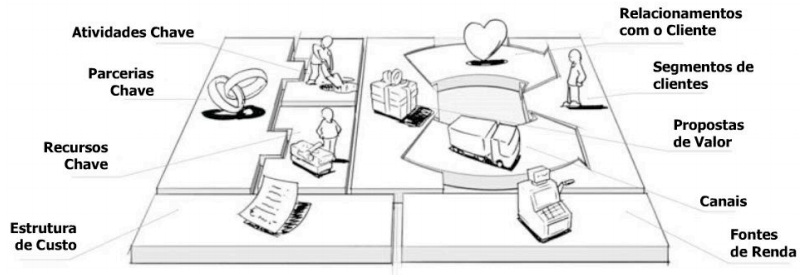
\includegraphics[width=0.95\textwidth]{./fig/BMC_Abstrato}
 \caption{Representação dos 9 blocos do modelo de negócio \cite{bmc2011}.}
 \label{fig:BMC_Abstrato}
\end{figure}

O canvas pode ser dividido em duas partes, um lado emocional, do lado esquerdo, que aborda questões relacionadas a relacionamento e interação entre os atores, e outro lado lógico/racional, no lado direito, cujo foco está na eficiência do processo \cite{bmcmoveis2013}. A proposição de valor está no centro, representando a razão para qual cada lado se desenvolve \cite{bmc2011}.

Os nove blocos básicos descritos na tabela \ref{tab:9blocos} compõem o modelo de negócio e estão inclusos dentro de quatro macro áreas: clientes (proposição de valor), oferta de valor (segmento de clientes, canais e relacionamento), infraestrutura (recursos principais, atividades-chave e principais parcerias) e viabilidade financeira (estrutura de custos e fontes de receita) \cite{bmc2011}. 

\begin{figure}[H]
 \centering
  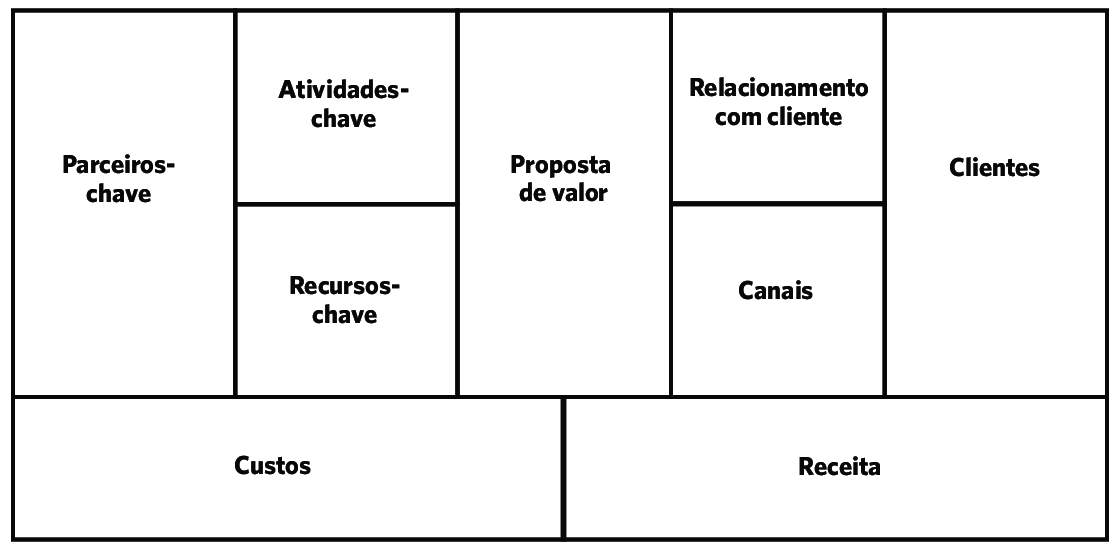
\includegraphics[width=0.90\textwidth]{./fig/estrutura_canvas}
 \caption{Ferramenta Business Model Canvas \cite{bmc2011}.}
 \label{fig:estrutura_canvas}
\end{figure}

% ######## init table ########
\begin{table}[H]
 \centering
% distancia entre a linha e o texto
 {\renewcommand\arraystretch{1.25}
 \caption{Os nove blocos do modelo de negócio e suas características \cite{bmctese2004} \cite{bmc2011}.}
 \label{tab:9blocos}
 \begin{tabular}{ l l }
  \cline{1-1}\cline{2-2}  
    \multicolumn{1}{|p{3.083cm}|}{\textbf{Bloco}} &
    \multicolumn{1}{p{7.283cm}|}{\textbf{Descrição}}
  \\  
  \cline{1-1}\cline{2-2}  
    \multicolumn{1}{|p{3.083cm}|}{\textbf{Proposição de valor}} &
    \multicolumn{1}{p{7.283cm}|}{Conjunto de produtos e serviços que criam valor para um segmento de cliente específico.}
  \\  
  \cline{1-1}\cline{2-2}  
    \multicolumn{1}{|p{3.083cm}|}{\textbf{Segmentos de cliente}} &
    \multicolumn{1}{p{7.283cm}|}{São os diferentes grupos de pessoas a quem uma organização deseja oferecer algo de valor.}
  \\  
  \cline{1-1}\cline{2-2}  
    \multicolumn{1}{|p{3.083cm}|}{\textbf{Canais}} &
    \multicolumn{1}{p{7.283cm}|}{São os meios empregados pela organização para manter contato com os clientes}
  \\  
  \cline{1-1}\cline{2-2}  
    \multicolumn{1}{|p{3.083cm}|}{\textbf{Relacionamento com clientes}} &
    \multicolumn{1}{p{7.283cm}|}{Tipo de relacionamento que a organização estabelece entre com seus clientes.  }
  \\  
  \cline{1-1}\cline{2-2}  
    \multicolumn{1}{|p{3.083cm}|}{\textbf{Recursos principais}} &
    \multicolumn{1}{p{7.283cm}|}{Descreve a organização das atividades e recursos que são necessários para criar valor para os clientes.}
  \\  
  \cline{1-1}\cline{2-2}  
    \multicolumn{1}{|p{3.083cm}|}{\textbf{Atividades-chave}} &
    \multicolumn{1}{p{7.283cm}|}{Habilidades em realizar as ações necessárias mais importantes para criar valor para os clientes. }
  \\  
  \cline{1-1}\cline{2-2}  
    \multicolumn{1}{|p{3.083cm}|}{\textbf{Parcerias principais}} &
    \multicolumn{1}{p{7.283cm}|}{Principais rede de fornecedores e os parceiros que fazem o modelo de negócio funcionar}
  \\  
  \cline{1-1}\cline{2-2}  
    \multicolumn{1}{|p{3.083cm}|}{\textbf{Estrutura de custo}} &
    \multicolumn{1}{p{7.283cm}|}{É a descrição de todos os custos envolvidos na operação do modelo de negócio. }
  \\  
  \cline{1-1}\cline{2-2}  
    \multicolumn{1}{|p{3.083cm}|}{\textbf{Fontes de receita}} &
    \multicolumn{1}{p{7.283cm}|}{Descreve a maneira como a organização ganha dinheiro através de cada segmento de cliente. }
  \\  
  \hline

 \end{tabular} }
\end{table}

%% - - - - - - - - - - - - - - - - - - - - - - - - - - - - - - - - - - -
\section{Fatores específicos}
\label{sec:temp}

Conforme Walker e Brown \cite{walkerebrown(2004)2004}, os fatores de sucesso estão diretamente ligados às características específicas de cada negócio. Em contrapartida, existem autores que não estudam aspectos do negócio em si, mas sim traços de personalidade do dirigente do empreendimento ou seus hábitos e práticas que podem levar ao sucesso do negócio \cite{criticalfactors2014}. Krauss \cite{krausss.i.etal2005}, por exemplo, analisa a orientação empreendedora do dirigente da pequena empresa que será composta por algumas características que influenciam positivamente o sucesso do negócio. 
\begin{itemize}
\item Orientação de aprendizagem: capacidade de aprender com as experiências;
\item Orientação para a realização/conquista: buscar feedback, orientação para o crescimento, assumir riscos;
\item Orientação para a autonomia: expressar sua individualidade no seu trabalho, dar valor a sua autonomia, tomada de decisões;
\item Agressividade competitiva: assertividade, afirmação, empenho, vontade de vencer;
\item Orientação para a inovação: mentalidade aberta para novas ideias no que diz respeito a produtos, serviços, administração e processos tecnológicos;
\item Assumir riscos: assumir riscos calculados (tendo em vista que o risco é inevitável);
\item Iniciativa Pessoal: pró-atividade e persistência.
\end{itemize}

%% - - - - - - - - - - - - - - - - - - - - - - - - - - - - - - - - - - -
\section{Fatores externos}
\label{sec:temp}

O macroambiente empresarial contêm fatores externos à empresa que apresentam variáveis situacionais que podem facilitar ou inibir o empreendedorismo na inicialização e durante o ciclo de vida das PME. Esses fatores apresentam oportunidades, ameaças e informações que afetam todos os empreendedores nesse ambiente, independentemente de sua formação, educação ou conceito de negócio \cite{Dahlqvist2000}. Fatores externos macroambientais não são controláveis e o sucesso da PME geralmente depende da capacidade do empresário de lidar com eles \cite{vivierss.vaneedens.&venter2001}. Abaixo é apresentado alguns fatores externos existentes.

\subsection{Fatores político institucionais}
\label{subsec:framing}

Nos países em desenvolvimento, o clima político e os requisitos legais para fazer negócios em um país podem ser um possível aprimorador ou um grande obstáculo ao desenvolvimento do empreendedorismo \cite{thandekaruthkunene2008}. Os programas de apoio às PMEs do governo, por exemplo, podem garantir que as PMEs recebam apoio contínuo na forma de conhecimento e experiência para garantir o crescimento dos negócios além da incubação inicial \cite{ligthelma.a.&cantm.c2002}. A falta de apoio do setor público tem um impacto negativo no desenvolvimento do empreendedorismo em um país.

Políticas, legislação, estruturas, regulamentos e leis macroeconômicas são fatores que podem facilitar ou dificultar o desenvolvimento do empreendedorismo. Políticas, regulamentos comerciais, trabalhistas e tributários adequados podem proporcionar um ambiente propício que incentive o investimento e a sustentabilidade dos empreendedores. Por outro lado, um ambiente externo hostil apresenta restrições legais e regulatórias que sufocam o empreendedorismo e aumentam os custos dos negócios \cite{ligthelma.a.&cantm.c2002}.

\subsection{Fatores socioculturais}
\label{subsec:framing}

As condições socioculturais refletem o estágio de desenvolvimento do país. Essas condições e aspectos sociais da cultura do país podem criar um ambiente propicio que beneficia as PMEs, ou podem apresentar pressões que sufocam o empreendedorismo.
\\
\\
\textbf{Acesso à infraestrutura pública de qualidade}
\\

O acesso a serviços públicos de infraestrutura física inclui água, eletricidade, estradas, telecomunicações, telefones, mídia eletrônica e serviços postais, cruciais para iniciação, desenvolvimento e crescimento de negócios. O acesso limitado a estes serviços é uma grande restrição à sobrevivência das PMEs e ao crescimento, pois limita as operações e restringe o acesso a mercados e matérias-primas \cite{thandekaruthkunene2008}.
\\
\\
\textbf{Acesso a dinheiro / capital}
\\

A disponibilidade de recursos econômicos apropriados é importante para o desenvolvimento dos negócios. Isso permite que as PMEs garantam a experiência e as matérias-primas necessárias para colocar em prática as idéias empreendedoras, sejam competitivas, sobrevivam em condições desfavoráveis e cresçam. A falta de capital e o acesso limitado ao financiamento é um fator que inibe o empreendedorismo e influencia negativamente o crescimento, pois impede o progresso que vem da aplicação pontual de recursos \cite{ligthelma.a.&cantm.c2002}.
\\
\\
\textbf{Acesso à tecnologia}
\\

A globalização, o acesso à tecnologia e as descobertas tecnológicas têm proporcionado um número crescente de empresas construídas com garantia de qualidade, inovações de alta tecnologia e propriedade intelectual. As PMEs precisam ter acesso a tecnologia apropriada para obter vantagem competitiva \cite{thandekaruthkunene2008}. 

Segundo o modelo TOE (Technology-Organization-Environment ou Tecnologia –
Organização – Ambiente externo) apresentado na figura \ref{fig:inovacaotec}, há três elementos que influenciam uma empresa no processo de adoção e implementação de uma inovação especificamente tecnológica. Um dos grandes desafios para as empresas atuantes na economia digital é a criação
de um clima organizacional no qual a inovação seja valorizada e estimulada \cite{rosanasantarosa2016}. 

\begin{figure}[hbt!]
 \centering
  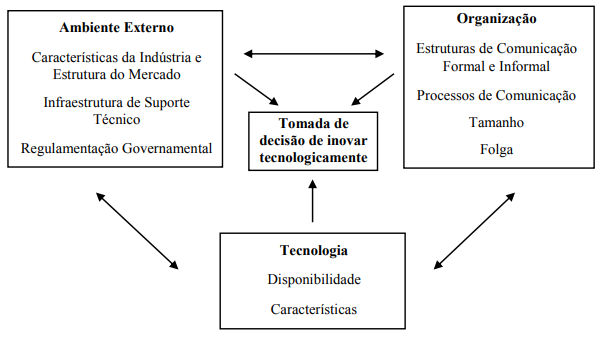
\includegraphics[width=0.8\textwidth]{./fig/inovacaotec}
 \caption{Modelo TOE (Tecnologia – Organização – Ambiente externo) \cite{rosanasantarosa2016}}
 \label{fig:inovacaotec}
\end{figure}

\begin{itemize}
\item O contexto tecnológico envolve as tecnologias relevantes, sua disponibilidade, características e práticas de uso. 
\item O contexto organizacional refere-se ao porte, processos de comunicação, qualidade e disponibilidade de recursos, estruturas formais e informais da empresa. 
\item O contexto de ambiente diz respeito às características da indústria de atuação, estrutura do mercado, infraestrutura técnica e regulamentação governamental.
\end{itemize}
\\
\\
\textbf{Valores, crenças e normas}
\\

Os valores, crenças e normas compartilhadas em uma sociedade são fatores contextuais importantes, pois, programam e afetam empreendedores em uma determinada comunidade, grupo étnico, região ou país, gerando assim, diferenças entre as fronteiras nacionais e regionais. Os níveis de atividade empreendedora em um país são afetados significativamente por estes fatores \cite{ligthelma.a.&cantm.c2002}.

\subsection{Fatores econômicos}
\label{subsec:framing}

O sucesso de um novo empreendimento depende do estado da economia nacional no momento em que o negócio é lançado. Exemplos são discutidos brevemente abaixo:
\\
\\
\textbf{Densidade de empresas}
\\

A densidade de empresas é definida como o número de empresas em uma determinada população e em um determinado momento e refere-se à porcentagem de empreendedores existentes e possíveis \cite{thandekaruthkunene2008}. Quanto menor a densidade de empresas naquele segmento, maiores serão as chances do negócio obter sucesso.
\\
\\
\textbf{Inflação}
\\

Inflação refere-se a um aumento contínuo e generalizado dos preços em uma economia e ela afeta significativamente o empreendedorismo, pois, com a inflação em alta significa que o valor da riqueza diminui, a população reduz o consumo e, portanto, há menos oportunidades para os empreendedores \cite{vivierss.vaneedens.&venter2001}.
\\
\\
\textbf{Desemprego}
\\

O desemprego afeta o processo de empreendedorismo. Onde há alto desemprego, muitas pessoas são levadas ao empreendedorismo para sobreviver e ao mesmo tempo por causa dessa alta do desemprego e renda limitada, os mercados se tornam naturalmente limitados \cite{ligthelma.a.&cantm.c2002}. Taxa de desemprego menor propiciará ao empreendedor uma condição favorável de mercado.

\subsection{Fatores de mercado}
\label{subsec:framing}

Fatores de mercado são fatores específicos do setor, associados ao setor em que a empresa opera e representam condições de mercado, interesses ou ações de consumidores, concorrentes, intermediários e fornecedores \cite{Dahlqvist2000}. Exemplos serão discutidos abaixo:
\\
\\
\textbf{Localização}
\\

A localização geográfica tem suas implicações no acesso a mercados e outros recursos, como finanças, mão de obra qualificada e infraestrutura \cite{Dahlqvist2000}. Para as PMEs esse fator pode ser crucial para a sobrevivência.
\\
\\
\textbf{Concorrência}
\\

Hoje, as PMEs operam em um contexto global caracterizado por competição intensificada. A concentração competitiva, juntamente com as ações e estratégias de mercado dos concorrentes, tem um impacto positivo ou negativo no processo empreendedor. Portanto, uma análise dos concorrentes e a tomada de ações para combater essa concorrência é crucial para a sobrevivência de uma PME \cite{ligthelma.a.&cantm.c2002}.
\\
\\
\textbf{Condições de mercado}
\\

A escolha de um segmento de mercado com potencial crescimento é um fator que influencia o sucesso das PME. Uma seleção de mercado ruim, por exemplo, com muitas imperfeições, muita heterogeneidade ou tamanho limitado de mercado com perspectivas de crescimento ruins, pode afetar negativamente o processo de empreendedorismo \cite{vivierss.vaneedens.&venter2001}. Portanto, ter acesso a conhecimentos sobre oportunidades em mercados específicos teria um impacto positivo no empreendedorismo.

%% - - - - - - - - - - - - - - - - - - - - - - - - - - - - - - - - - - -
\section{Fatores internos}
\label{sec:temp}

O ambiente interno tem impacto no empreendedorismo e no sucesso dos negócios. O ambiente interno inclui todos os fatores específicos da empresa que são influenciados por ações específicas praticados por ela, incluindo a disponibilidade de recursos e habilidades pessoais para exercer funções empresariais e o uso efetivo de recursos dentro da empresa. As deficiências no ambiente interno são a principal causa de falhas nas PMEs, com mais de 65\% das causas de falhas \cite{ligthelma.a.&cantm.c2002}.

\subsection{Características do empreendedor}
\label{subsec:framing}

As características do empreendedor, como traços, valores e atitudes são frequentemente citadas como os fatores mais influentes relacionados ao desempenho de uma PME e sua competitividade. Estudos anteriores do processo empreendedor examinaram a chamada personalidade empreendedora ou um único perfil psicológico do empreendedor para encontrar traços individuais de empreendedores bem sucedidos em comparação com não empreendedores.

Embora não exista um perfil de personalidade abrangente, acredita-se amplamente que existem certas características necessárias para cumprir as tarefas e os desafios da criação de novos empreendimentos e sem os quais o processo empreendedor paralisa e acaba atrofiando. Quanto mais próxima a correspondência entre as características pessoais do indivíduo e os requisitos característicos de ser um empreendedor, mais bem sucedido será o indivíduo \cite{thandekaruthkunene2008}.
\\
\\
\textbf{Lócus de controle interno}
\\

Uma das características consistentemente encontradas em empreendedores bem sucedidos é a tendência para o empreendedor ter lócus de controle interno. Esse controle refere-se ao grau em que um indivíduo percebe que o resultado de um evento está dentro ou fora de seu controle pessoal. Uma pessoa com lócus de controle interno acredita que ele tem influência sobre os resultados por meio de sua capacidade, esforço ou habilidades. Por outro lado, pessoas com lócus de controle externo acreditam que forças externas como sorte, destino ou poderosas outras pessoas controlam e determinam resultados \cite{stephenl.muelleranisyas.thomas2001}.
\\
\\
\textbf{Adaptação à mudança}
\\

Quando os proprietários consideram seu ambiente desestabilizador, a adaptação e a flexibilidade tornam-se uma estratégia crítica para o sucesso do empreendimento. Uma resposta intolerante à mudança pode levar à negação, comportamento que evita riscos e imposição de restrições e estruturas arbitrárias que sufocam a capacidade de adaptação do proprietário \cite{MorrisMichaelandZahra2000}. A adaptação é crucial para o desempenho dos negócios.
\\
\\
\textbf{Iniciativa}
\\

Ter iniciativa é essencial, pois o negócio depende das ações do empreendedor. Muitas pessoas que consideram uma oportunidade empreendedora desejável e viável simplesmente nunca conseguem realizar atividades essenciais para
iniciar o negócio devido a paralisia alimentada por inércia, preguiça, dúvida, medo, entre outros \cite{stephenl.muelleranisyas.thomas2001}.
\\
\\
\textbf{Propensão a assumir riscos}
\\

A capacidade de assumir riscos é uma das características definidoras de um empreendedor. O risco é definido como a possibilidade de se obter resultados indesejados \cite{MorrisMichaelandZahra2000}. A propensão a assumir riscos combina todos os fatores que lidam com riscos, incluindo correr riscos calculados e ser realista ao analisar as oportunidades.

Os empresários enfrentam incertezas e possíveis riscos em pelo menos cinco áreas principais, incluindo financeira, profissional, famíliar, social e psicológica. Os empresários de PME bem sucedidos tendem a assumir riscos moderados, que fazem avaliações de risco calculadas e não têm medo de falhar. As PMEs mal sucedidas não planejam contingências e dependem apenas da sorte, o que é considerado imprudente \cite{thandekaruthkunene2008}.
\\
\\
\textbf{Capacidade de aprender}
\\

Os empreendedores de sucesso têm capacidade de absorção e capacidade de aprender. A aprendizagem refere-se à aquisição de conhecimento por atores dispostos e capazes de aplicar esse novo conhecimento na tomada de decisões ou na influência de outros na organização \cite{MorrisMichaelandZahra2000}.

\subsection{Características da empresa}
\label{subsec:framing}
Características da própria empresa que devem ser levados em consideração. Abaixo será apresentado alguns.
\\
\\
\textbf{Controle de estoque}
\\

Um sistema de controle eficaz mantém os negócios rastreados e alerta os gerentes sobre qualquer perigo em potencial. O maior investimento que uma pequena empresa faz é em estoque, mas o controle de estoque é uma das responsabilidades gerenciais mais negligenciadas. Níveis de estoque insuficientes resultam em escassez e falta de estoque, causando insatisfação e perda dos clientes. A situação mais comum é que a empresa tem produtos em estoque, só que de um produto que deveria ter na quantidade mínima. Muitas pequenas empresas que falham devido ao mau controle de estoque, têm quantidades excessivas de dinheiro vinculadas a um estoque inútil acumulado \cite{palukukazimoto2009}.
\\
\\
\textbf{Planejamento}
\\

Muitos empreendedores não percebem a importância do planejamento para o sucesso de suas empresas. Frequentemente, os gerentes de pequenas empresas negligenciam o processo de planejamento porque pensam que é algo que beneficia apenas as grandes empresas. O não planejamento do futuro de uma empresa terá um efeito devastador sobre a existência dela no futuro. Isso geralmente é ocasionado por dois fatores, a falta de planos estratégicos e a expansão não planejada. A expansão da empresa deve ser financiada pelos lucros acumulados ou pelas contribuições de capital dos proprietários. À medida que a empresa aumenta em tamanho e complexidade, os problemas tendem a aumentar em proporção e os gerentes precisam aprender a lidar com isso \cite{palukukazimoto2009}.
\\
\\
\textbf{Politica de preços}
\\

Os empreendedores precisam estabelecer preços que obtenham os lucros necessários, primeiro entendendo o quanto custa produzir, comercializar e entregar seus produtos e serviços. Os proprietários de pequenas empresas geralmente subestimam seus bens e serviços, resultando em perdas que acabam causando seu fracasso \cite{thandekaruthkunene2008}. Estabelecer como objetivo principal uma estratégia de preços competitivos para atrair clientes pode representar um risco, como podemos observar na figura \ref{fig:precos}.

\begin{figure}[hbt!]
 \centering
  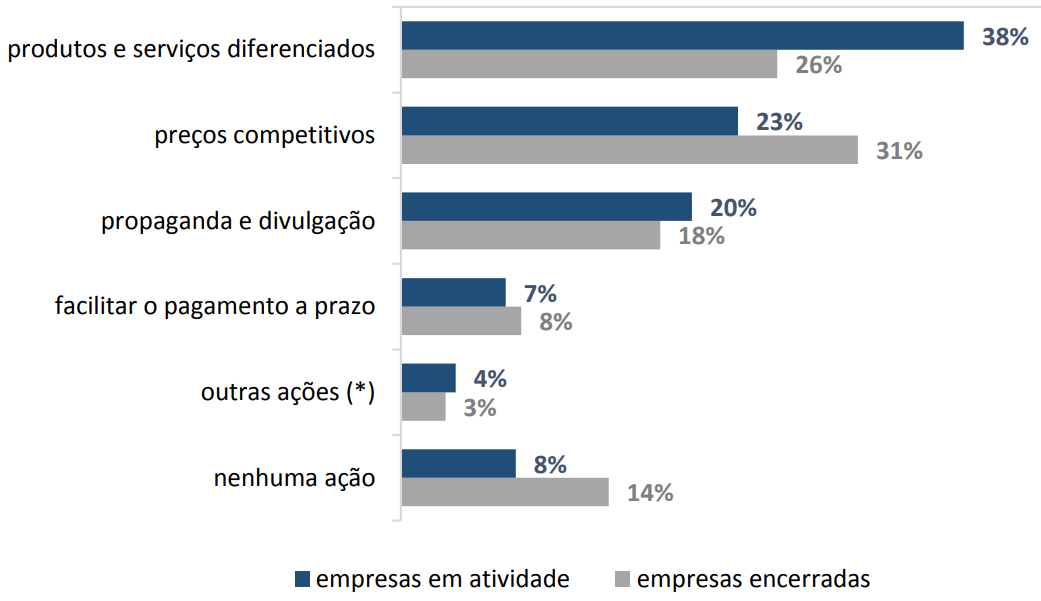
\includegraphics[width=0.70\textwidth]{./fig/precos}
 \caption{Estratégia para atrair clientes \cite{sebraesp}}
 \label{fig:precos}
\end{figure}

\subsection{Experiência}
\label{subsec:framing}

Quanto maior a experiência anterior dos empreendedores, maior será sua qualidade empreendedora, pois a experiência envolverá um processo de aprendizado que o ajudará a identificar oportunidades, reduzir sua ineficiência inicial e também melhorar sua capacidade de executar várias tarefas. A experiência anterior inclui experiência de trabalho, experiência em gerenciamento de negócios e experiência específica do setor \cite{thandekaruthkunene2008}.
\\
\\
\textbf{Experiência de trabalho}
\\

A capacidade de assimilar e aprender com a própria experiência é um dos principais fatores que influenciam o processo empreendedor. A maioria das novas empresas é iniciada por pessoas que trabalharam em outros empregos que lhes deram a experiência relevante para identificar uma oportunidade de negócios e a capacidade técnica de produzir o produto ou prestar o serviço identificado. Pessoas sem experiência de trabalho têm menos recursos e podem achar mais difícil desenvolver uma boa ideia de negócio. Sem experiência profissional, muitas das PMEs permanecem no estágio de sobrevivência ou estão fadadas ao fracasso desde o início \cite{thandekaruthkunene2008}.
\\
\\
\textbf{Experiência como proprietário de um negócio}
\\

A experiência empreendedora pode ser vista como um colaborador significativo do capital humano empreendedor, pois pode se traduzir em conhecimento valioso desenvolvido por meio da experiência direta. Essa experiência pode construir reputações que ajudam a proteger recursos e ativos que podem ser utilizados na identificação e exploração de empreendimentos subsequentes \cite{guzmanj.&santosf.j.2001}. As PMEs que iniciam seus negócios sem nenhuma experiência anterior como proprietário de empresas precisam arcar com os custos de adquirir habilidades empreendedoras enquanto implementam a ideia.
\\
\\
\textbf{Experiência específica}
\\

Ter experiência profissional em uma organização que está no mesmo setor em que o empreendedor inicia seu novo empreendimento pode aumentar a probabilidade de sobrevivência e alto desempenho \cite{Dahlqvist2000}. A experiência específica no setor é uma maneira essencial de adquirir habilidades e conhecimentos para responder a uma necessidade percebida do mercado, além de obter importantes contatos comerciais e insights sobre o setor \cite{guzmanj.&santosf.j.2001}. Esse conhecimento é principalmente demorado e caro de se construir.

\subsection{Capital humano}
\label{subsec:framing}

Capital humano pode ser definido como atitudes, comprometimento, valores, conhecimento, experiência, educação, capacidade e habilidades que ajudam o empreendedor e sua equipe nas tarefas de iniciar, administrar e expandir um negócio \cite{raucha.&fresem2000}. Os fatores de capital humano que influenciam o sucesso ou o fracasso de novos empreendimentos envolvem o histórico do empreendedor, suas ações, as decisões que eles tomam, as estratégias que desenvolvem e o estilo de liderança que exercem. 

Elas estão relacionadas às motivações dos empreendedores, e a equipe de gerentes e funcionários que reúnem. Selecionar um grupo de pessoas pode ser uma tarefa dificil, como é apresentado na figura \ref{fig:dificuldadedecontratar}. O capital humano do empreendedor é uma combinação de fatores, que podem ter um efeito positivo ou negativo na produtividade \cite{thandekaruthkunene2008}.

\begin{figure}[hbt!]
 \centering
  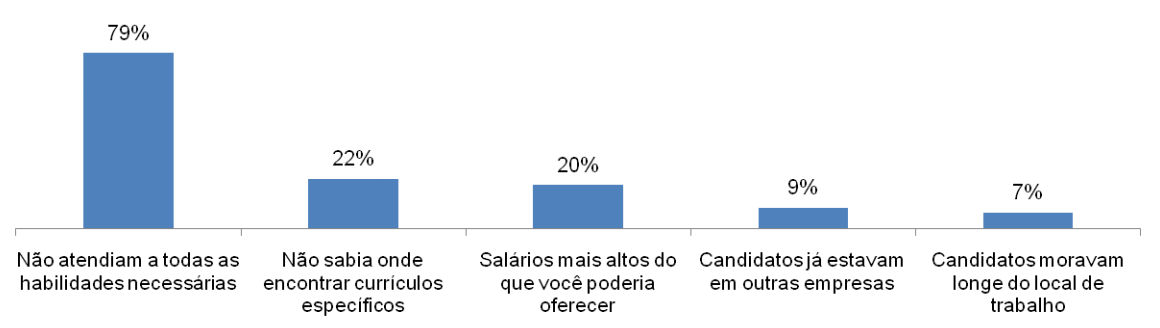
\includegraphics[width=1.00\textwidth]{./fig/dificuldadesdecontratar}
 \caption{Dificuldades para se contratar \cite{ecommerceschool2015}.}
 \label{fig:dificuldadedecontratar}
\end{figure}

%% - - - - - - - - - - - - - - - - - - - - - - - - - - - - - - - - - - -

\section{Fatores para Modelos de Negócio Online}
\label{sec:model}

Fatores influenciadores são as poucas áreas no qual a empresa deve se fortalecer. A identificação destes fatores é feita através da atividade principal do negócio, das áreas onde esta a maior concentração de dinheiro e dos setores que impactam nos lucros \cite{criticalfactors2014}. Abaixo apresentamos alguns fatores identificados.

%Conhecimento de TI
\subsection{Conhecimento sobre TI}
\label{subsec:conhecimentoti}

O conhecimento sobre TI representa um papel importante na adoção de novas tecnologias e aumenta o grau de adoção e desempenho de tecnologia da empresa. Especialistas em negócios na empresa possibilita que ela participe de inovações de TI, já que poderiam desenvolver sua própria plataforma de vendas ou poderiam usar tecnologias específicas para gerenciar melhor a cadeia de valor \cite{criticalfactors2012}.

%Terceirização
\subsection{Terceirização}
\label{subsec:terceirizacao}

A terceirização pode melhorar o desempenho das empresas que não têm conhecimentos ou não querem gastar seus recursos internos em certas áreas. Geralmente, a principal razão para um empresa terceirizar uma função específica é a falta de recursos humanos e experiência para isso.

Ela é feita frequentemente pelas PMEs porque pode resolver o problema da limitação de recursos intelectuais. A terceirização pode ser uma solução eficaz para melhorar o desempenho destas empresas, que geralmente sofrem com a falta de conhecimento e os altos custos iniciais de gerenciamento do negócio \cite{criticalfactors2012}. 

Possuir e operar recursos de TI por exemplo pode parecer prático em grandes corporações, mais a infraestrutura de TI terceirizada será uma alternativa competitiva melhor e mais econômica para pequenas empresas, pois oferece muitos benefícios, como baixo custo de instalação e manutenção. Estes serviços geralmente possuem suporte profissional 24 horas por dia, backup de dados, largura de banda ilimitada, atualizações regulares de software e hardware e o principal, a flexibilidade para escalar operações rapidamente para atender a surtos repentinos na demanda por serviços e baixo risco de falha de serviço \cite{terc2009}.

%Uso do marketplace
\subsection{Marketplace}
\label{subsec:framing}

O marketplace surgiu no Brasil em 2012 e é conhecido como uma espécie de shopping center virtual. No marketplace o lojista faz o cadastro dos produtos informando a descrição e enviando as fotos. A cada busca feita pelos consumidores, uma listagem de anúncios é obtida, incluindo os itens da empresa. O ranqueamento dessa lista possui diversos critérios de elevação ou queda na exposição de cada anúncio, variando de acordo com cada marketplace.

Esse segmento ganha mercado a cada ano que passa, porque é um modelo de negócio que atrai empresas de diversos setores e consumidores de diversos mercados. Com isso, temos uma variedade enorme de produtos, suprindo a demanda de consumo inicial e até despertando o interesse para itens que não estavam na lista de compras do consumidor \cite{ecombrmkt}.

Nesse marketplace, o consumidor interessado em comprar algum produto ou serviço pode consultar a disponibilidade daquilo que ele deseja, fazer a encomenda e executar as transações financeiras. Logo após, essas transações são processadas pelo operador do marketplace, que repassa a porcentagem combinada do valor das vendas para a empresa.

O pequeno lojista que não teria muitos acessos em uma loja virtual própria, passa a ganhar mais visibilidade. Além do mais, ele pode acompanhar suas métricas dentro do marketplace, assim, ele pode identificar as melhores práticas, tendências e soluções para problemas que possam estar afetando o desempenho da empresa \cite{marktsebrae}.

Para ser encontrado na internet é preciso investir em anúncios, utilizando o Google, Facebook e outras ferramentas digitais. Com o crescimento da concorrência o valor desses anúncios cresce a cada dia. O Marketplace oferece valores menores, com uma porcentagem fixa sobre os produtos vendidos, o que seria essencial para o micro e pequeno empresário \cite{marktecbr}.

%Cross docking
\subsection{Cross docking}
\label{subsec:framing}

Cross docking é um método de logística em que o gestor não precisa necessariamente armazenar os produtos na sua empresa. No momento em que um pedido é realizado, ele envia uma solicitação de compra para o fornecedor, que por sua vez vai enviar para ele as mercadorias. Ao aproximar essa realidade para as pequenas e médias empresas o capital a ser utilizado para aquisição e gerenciamento do estoque pode ser empregado em outros investimentos ou revertido para outras áreas da empresa. A empresa Privalia por exemplo, que é uma loja virtual multimarcas, não possui um item dos produtos que vende. O consumidor final faz o pedido no site, a fábrica envia para o centro de distribuição e, de lá é enviado ao consumidor.

Neste contexto seriam necessários investimentos principalmente na automação de informação para toda a cadeia operacional, como por exemplo, dados de pedido, de vendas, previsão de chegada, disponibilidade do item, etc. Para que o cross docking funcione é necessário realizar um planejamento correto para que a gestão do fluxo constante de carga funcione como um controle preventivo da ruptura do abastecimento. E um dos elementos mais importantes é a confiança nos parceiros, como fornecedores, principalmente nos quesitos qualidade do produto e garantia de entrega \cite{sebraecross}.

%Segmentação do negócio
\subsection{Segmentação}
\label{subsec:framing}

O maior desafio dos empresários é construir uma marca diferenciada em meio a grandes players já consolidados no meio digital. Para enfrentar esse desafio, é preciso identificar o perfil médio do consumidor 2.0, aquele que cada vez mais adere a serviços personalizados na internet. Para se encaixar no perfil de consumo desses novos consumidores a oferta de produtos e serviços deve ser cada vez mais afunilada. 
%\cite{nichoexame}.

Um negócio segmentado é a melhor opção para se iniciar uma operação online, uma vez que necessita de menos investimento em marketing e tecnologia. Atuar num mercado de nicho permite que a empresa assuma um posicionamento mais preciso, o que facilita a comunicação com os clientes e a criação de uma imagem forte no segmento. Os consumidores se sentem mais confortáveis para comprar em uma loja de nicho, além do mais, eles preferem resolver o problema de uma forma mais agíl, nem que tenha que pagar um valor adicional \cite{nichoNV}.

No setor de comércio eletrônico por exemplo, os principais casos de sucesso de pequenas e médias empresas estão ligados a negócios que escolheram nichos de atividade ou segmentos de mercado os quais os seus empreendedores dominavam. É o caso da loja Flores Online, que começou como uma pequena empresa vendendo um produto inusitado: flores pela Internet. Desta forma, alcançou sucesso com o seu modelo de vendas inovador com foco na qualidade do seu produto e excelência no atendimento ao cliente. Outro exemplo é a loja online DOC CHECK SHOP, fundada em 1996, a DocCheck Medizinbedarf und Logistik GmbH vende acessórios médicos na Europa, com o crescimento agora possui 7 lojas online em quatro idiomas \cite{nichobraeur}.

% Implantar a melhoria continua dos processos
\subsection{Melhoria contínua}
\label{subsec:bpr}

O Business process reengineering (BPR), é a análise e redesenho de processos de uma empresa. Ele usa a tecnologia da informação para mudar e automatizar processos organizacionais, com o objetivo de alcançar maior eficiência operacional e prontidão para lidar com o rápido crescimento do volume de transações. É uma abordagem bastante utilizada em grandes empresas. Nas PMEs as restrições financeiras restringem o trabalho do BPR a um nível mais baixo e mais restrito, embora estudos mostrem que as PMEs podem se beneficiar igualmente do BPR porque os processos de negócios estão no coração do empreendimento \cite{terc2009}.

% KPI
\subsection{Indicador de desempenho}
\label{subsec:kpi}

A sigla KPI representa a junção das 3 primeiras letras das palavras Key Performance Indicator, que pode ser entendido como um indicador chave de desempenho. Segundo Parmenter \cite{parmenter}, os KPIs podem ser representados pela combinação de um ou mais indicadores, e representam um conjunto de medidas focadas nos aspectos mais críticos para o desempenho satisfatório e atingimento dos objetivos organizacionais, como mostrado na tabela \ref{tab:kpi}. 

É impossível definir indicadores universais, visto que cada tipo de negócio e, até mesmo, os departamentos de uma empresa precisam analisar dados diferentes. Dentre os principais indicadores, temos o que calcula o ticket médio, que é o valor médio que os clientes gastam cada vez que realizam uma compra na empresa. Para calcular basta dividir o valor total faturado pela quantidade de pedidos feitos \cite{locaweb2019}.

Outro indicador importante é o ROI, retorno sobre investimento, que irá revelar se um investimento gerou um faturamento suficiente para cobrir os próprios custos. Assim, é possível avaliar se vale a pena repetir a ação no futuro ou se ela não teve o retorno esperado. Temos também o CAC, Custo de aquisição de clientes, que calcula o valor que a empresa precisou investir para conquistar cada cliente \cite{locaweb2019}. 

Efetuar a gestão da empresa utilizando KPIs é um diferencial competitivo, e
um fator crucial para a sobrevivência e crescimento no cenário em que a concorrência
está cada vez maior e os clientes mais exigentes, pois permite que as estratégias
sejam implementadas e constantemente verificadas e atualizadas \cite{kpiufu2017}.

\begin{table}[]
 \centering
% distancia entre a linha e o texto
 {\renewcommand\arraystretch{1.25}
 \caption{Métricas para medir o objetivo de desempenho em uma empresa de software. \cite{kpiufu2017}}
 \label{tab:kpi}}
 
\begin{tabular}{|c|c|}
\hline
\textbf{\begin{tabular}[c]{@{}c@{}}Objetivo de \\ desempenho\end{tabular}} & \textbf{Possíveis métricas} \\ \hline
Qualidade & \begin{tabular}[c]{@{}c@{}}Nível de reclamação do consumidor; tempo médio entre falhas; \\ número de defeitos por unidade\end{tabular} \\ \hline
Velocidade & \begin{tabular}[c]{@{}c@{}}Tempo de resposta ao consumidor; tempo de ciclo; \\ frequência de entregas.\end{tabular} \\ \hline
Confiabilidade & \begin{tabular}[c]{@{}c@{}}Porcentagem de pedidos entregues com atraso; \\ aderência a programação.\end{tabular} \\ \hline
Flexibilidade & \begin{tabular}[c]{@{}c@{}}Tempo para mudar programações; \\ tempo de mudança de máquina.\end{tabular} \\ \hline
Custo & \begin{tabular}[c]{@{}c@{}}Custo por hora de operação; produtividade da mão de obra; \\ variação contra o orçamento.\end{tabular} \\ \hline
\end{tabular}
\end{table}

% Parcerias
\subsection{Parcerias}
\label{subsec:framing}

Nas pequenas empresas a parceria é particularmente importante porque a escassez de recursos faz com que eles trabalhem com estreita participação de fornecedores e parceiros comerciais. Atuando em conjunto as empresas podem alavancar o reconhecimento da marca, melhorar a eficácia do marketing, lançar produtos personalizados, aproveitar novas oportunidades de mercado e agilizar suas operações. Pode ser primordial para as pequenas empresas considerarem aderir a uma comunidade empresarial, porque a adesão pode levar a novos negócios e parcerias potenciais \cite{terc2009}.

% Inbound marketing
\subsection{Inbound marketing}
\label{subsec:framing}

Atualmente os consumidores têm se desvencilhado do antigo modelo de marketing. Com novas formas de acesso a novos conteúdos, os consumidores têm evitado a publicidade excessiva ou não desejada. O inbound marketing se diferencia das demais técnicas de marketing porque ao invés de interromper o cliente em potencial, a ideia é atraí-lo por meio de conteúdo relevante com a criação de conteúdos e sua distribuição através de blogs, das redes sociais e de campanhas de e-mail marketing. O objetivo é conquistar e manter leads, que consistem em contatos que poderiam ser convertidos em clientes \cite{inbci}, conforme é mostrado na Figura \ref{fig:inboundmarketing}.  

Geralmente o inbound marketing exige menores investimentos e oferece um bom retorno, quando trabalhadas de maneira profissional. Empresas que aderem a esse tipo de estratégia recebem mais oportunidades de venda. Portanto, ao se analisar a estrutura e recursos disponíveis nas pequenas e médias empresas e no cenário em que se insere o consumidor moderno, pode-se afirmar que o Inbound Marketing oferece bons recursos e os mais efetivos resultados para criar um entendimento sólido sobre o negócio para os potenciais consumidores \cite{inbpme}.

\begin{figure}[hbt!]
 \centering
  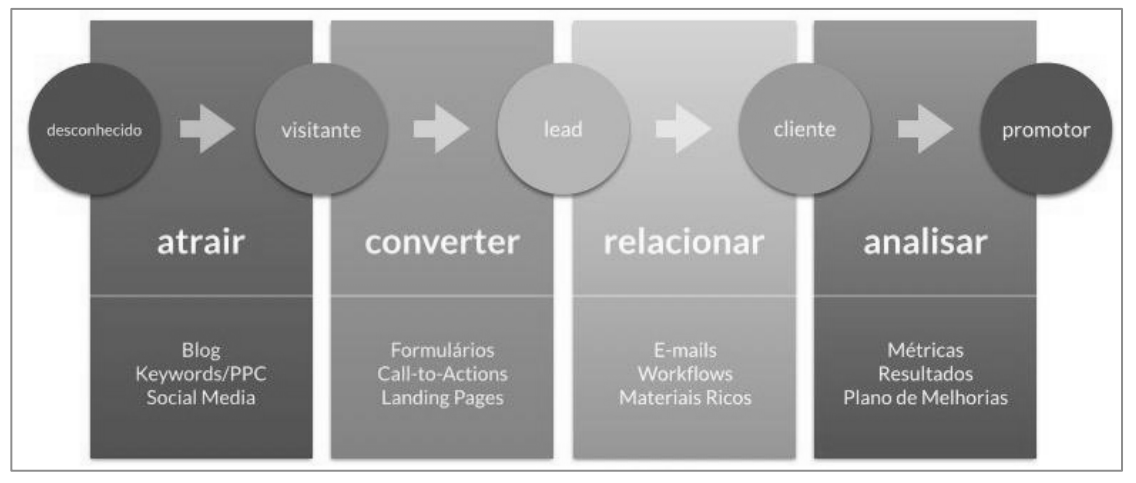
\includegraphics[width=0.90\textwidth]{./fig/inboundmarketing2}
 \caption{Ações do Inbound Marketing \cite{inbci}}
 \label{fig:inboundmarketing}
\end{figure}

\chapter{Metodologia}
\label{cap:texto}

Trata-se de um estudo exploratório, feito através de uma revisão bibliográfica com fontes secundárias e posteriormente com pesquisa quantitativa. A população alvo deste projeto de estudo são empresas de pequeno e médio porte que atuam de forma eletrônica. As buscas foram realizadas em sua maioria nas seguintes bases de dados bibliográficas: Google Scholar, SciELO, Periódicos Capes, ArXiv e Microsoft Academic. Ao finalizar as pesquisas em cada base, as referências duplicadas foram excluídas. 

Foram selecionados artigos publicados entre 2000 e 2019 (incluindo aqueles disponíveis online em 2019 que poderiam ser publicados em 2020), escritos em inglês, português ou espanhol. Optou-se pela busca por termos livres, com essa estratégia, houve uma recuperação de um número maior de referências, garantindo a detecção da maioria dos trabalhos publicados dentro dos critérios pré-estabelecidos. Os termos e-business; modelo de negócio; SME digital business; e critical success factors foram combinados com as associações e desfechos de interesse.

\section{Coleta de dados para a pesquisa}
\label{sec:figs}
 
Para obter uma amostra foi definida uma população alvo. A população alvo é o grupo ou os indivíduos a quem a pesquisa se aplica. Idealmente, a população alvo foi representada por uma lista de 285 empresas. A ferramenta para coleta de dados é um questionário estruturado que busca identificar o quanto estas empresas estão aderentes aos fatores habilitadores identificados.

Os questionários foram distribuídos via e-mail para empresas que de alguma forma atuam em parceria com o Instituto de Informática da Universidade Federal de Goiás. Foram aplicados também questionários em um workshop promovido pelo Instituto de Informática, em que foi apresentado a comunidade empresarial a Lei Geral de Proteção de Dados. As empresas também foram contatadas de forma aleatória por conveniência, validando a participação daquelas que concordaram em fazer parte do estudo colaborativamente.

A pesquisa de opinião aplicada ficou acessível na ferramenta Google forms por 29 dias, de 10/10/2019 a 07/11/2019, através do link: https://forms.gle/G5Pafno4JrR7NCpz7. Da relação total de convidados via e-mail, 41 responderam ao formulário, resultando em índice de retorno dos questionários de 15,41\%, o que pode ser considerado um número baixo, dado que para Marconi e Lakatos, questionários que são enviados para os entrevistados alcançam em média 25\% de devolução \cite{marconilakatos2005}. Dentre as principais desvantagens das pesquisas on-line podemos considerar a baixa taxa de resposta aos questionários \cite{henrique2010}.

Ao todo obteve-se 58 questionários respondidos, seja através dos questionários on-line e aplicação dos questionários presenciais. Algumas respostas foram dadas por indivíduos pertencentes a mesma organização, por isso houve a ocorrência de mais de um respondente para uma mesma empresa, reduzindo assim para um total de 55 questionários de pesquisa considerados válidos.


\section{Análise estatística}
\label{sec:figs}

O tratamento dos dados se dará através da ferramenta Excel, Google Sheets e do classificador do programa Weka 3, em que as respostas serão organizadas e, em seguida, através de tabelas e gráficos serão exibidas as informações provenientes das respostas coletadas. 

Do total de questionários considerados válidos, 15 responderam que não comercializam produtos/serviços em canais eletrônicos e 40 disseram que a empresa comercializa seus produtos/serviços em canais eletrônicos (e-commerce). Desta forma, com base nos resultados obtidos destas 40 empresas, foram feitos alguns gráficos para representar as informações, como mostrado no próximo capítulo.






\chapter{Análise e Discussão dos Resultados}
\label{cap:results}

Com base nos resultados obtidos na pesquisa aplicada aos empresários/gestores, caracterizados como público alvo, foi feita a análise dos dados, buscando a correlação dos fatores habilitadores identificados com as características de empresas que possuem um tempo de atuação no mercado considerado acima da média. 

\section{Análise dos resultados}
\label{subsec:framing}

Do total de empresas que comercializam produtos/serviços on-line, 94,9\% foram representadas por PMEs e 5.1\% por startups. Essas empresas relataram em sua maioria que preferem divulgar/comercializar seus produtos/serviços nas redes sociais com 87.5\%, seguido pela escolha do marketplace, com 60\%, como mostrado na Figura \ref{fig:plataformas}.

% Imagem fixa
\begin{figure}[h]
 
\centering
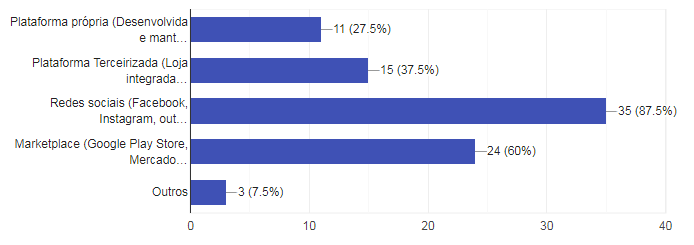
\includegraphics[width=14cm]{./fig/plataformasusadas}
\caption{Plataformas que as empresas divulgam/comercializam produtos/serviços on-line. (Fonte: Autoria própria, 2019)}
\label{fig:plataformas}
\end{figure}

A maioria da empresas consultadas na pesquisa possuem de 1 a 6 anos de atuação no mercado, representando 33,3\%, logo após temos as empresas com até 1 ano de atuação, com 28,2\%. As organizações com mais de 6 anos de atuação, representaram 25,6\% do total de entrevistados. Os gestores em sua maioria, informaram possuir nível de conhecimento em tecnologia da informação considerado razoável, com 46,2\%, como mostrado na figura \ref{fig:tempodemercado}. 

% Duas imagens -------------
\begin{figure}[H]
\center
\subfigure[08][Tempo de mercado.]{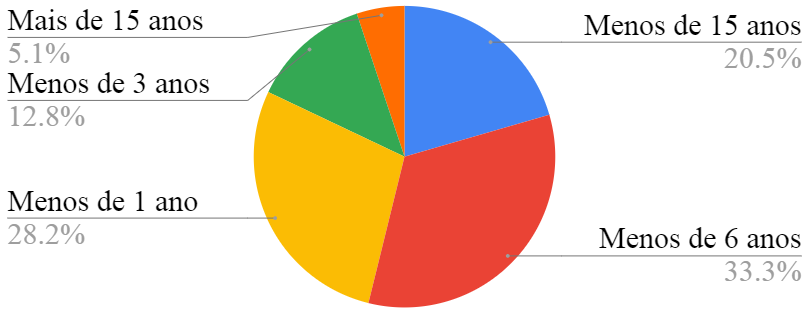
\includegraphics[width=7cm]{./fig/idade}}
\qquad
\subfigure[10][Nível de conhecimento em tecnologia da informação.]{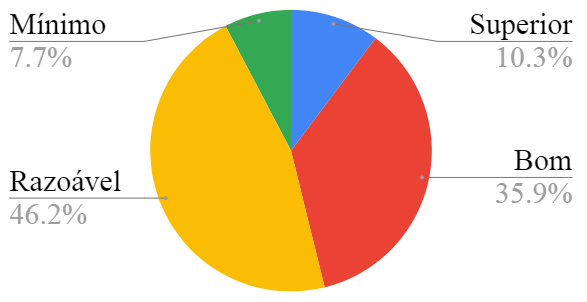
\includegraphics[width=5.5cm]{./fig/conhecimentoemti}}
\caption{Questões 8 e 10. (Fonte: Autoria própria, 2019)}
\label{fig:tempodemercado}
\end{figure}

As empresas em sua maioria terceirizam alguma função específica, recurso ou infraestrutura de TI, representando 61,5\%, o restante, 38,5\% optam por não tercerizar. A maior parte delas, 64,1\%, informaram que não utilizam o método cross docking para o gerenciamento de estoque de sua empresa, o que já era esperado, pois a maioria delas atua no mercado de desenvolvimento de software e na área de prestação de serviços.

Grande parte das empresas, representando 56,4\%, relataram que mapeiam o perfil do consumidor e atuam em um mercado de nicho, segmentado. Os empresários/gestores entrevistados, em sua maioria, com 61,5\%, realizam a análise ambiental e promovem estudos de redesenho (pivotar) dos processos da empresa regularmente.

Dentre as organizações, 59\% informaram que utilizam algum instrumento indicador que monitora e acompanha o nível de desempenho (KPIs, satisfatório, ou insatisfatório) e o nível de atingimento dos objetivos organizacionais (KRIs), 41\% não utilizam instrumento indicador em sua empresa. A maioria das empresas consultadas, 72,5\%, não estão inseridas em alguma comunidade empresarial, seja ela cooperativa ou associativa.

A maior parte das organizações, com 79,5\%, atuam na criação de conteúdo relevante e o distribui em redes sociais e campanhas de e-mail marketing. 61,5\% dos entrevistados fazem o acompanhamento durante o período de pós-venda, monitorando o feedback dos clientes na internet, tanto em redes sociais como sites de reclamação, para poder melhorar um produto/serviço.

Foi constatado que as pessoas que possuem nível de conhecimento em tecnologia da informação “Bom” ou “Superior”, estão, em sua maioria em empresas que possuem maior tempo de mercado, ou seja, acima de 3 anos de atuação. A maioria das pessoas que declaram possuir nível de conhecimento em tecnologia da informação “razoável” estavam presentes em empresas com menos de 1 ano de atuação. As empresas com mais de 15 anos de atuação possuem pessoas com nível de conhecimento em tecnologia da informação considerado “bom”, conforme a figura \ref{fig:grafico48}.

% Imagem fixa
\begin{figure}[H]

\centering
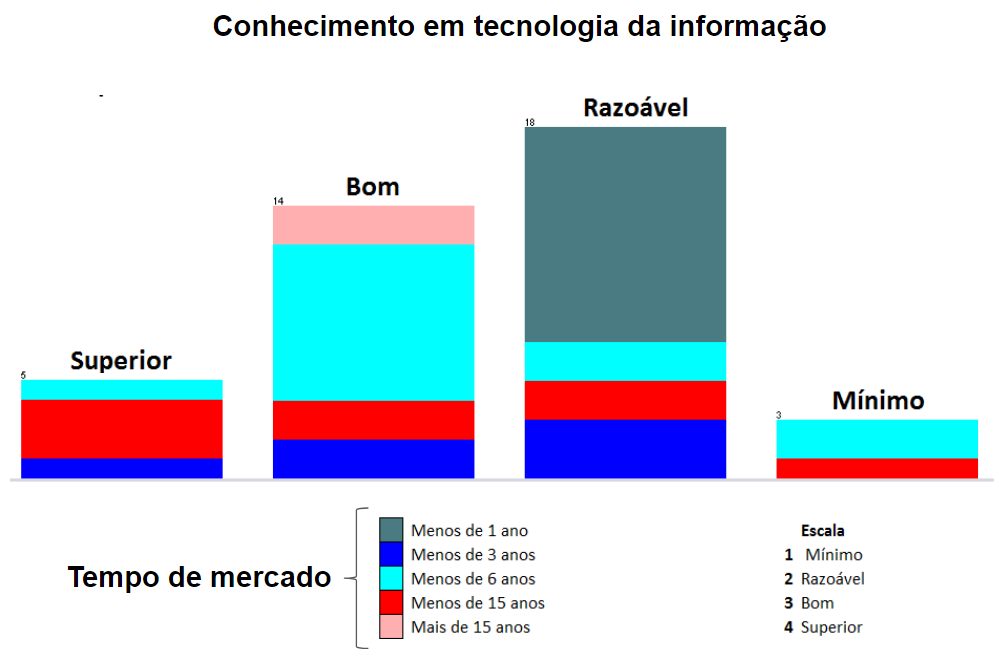
\includegraphics[width=13cm]{./fig/grafico01}
\caption{Conhecimento em TI X Tempo de mercado. (Fonte: Autoria própria, 2019)}
\label{fig:grafico48}
\end{figure}

As empresas que utilizam algum instrumento indicador que monitora e acompanha o nível de desempenho (KPIs, satisfatório, ou insatisfatório) e o nível de atingimento dos objetivos organizacionais (KRIs) são as que possuem maior tempo de mercado. As empresas com menos de 1 ano de atuação estão em sua maioria no grupo que não utilizar nenhum instrumento indicador, conforme mostrado na figura \ref{fig:grafico49}.

% Imagem fixa
\begin{figure}[H]

\centering
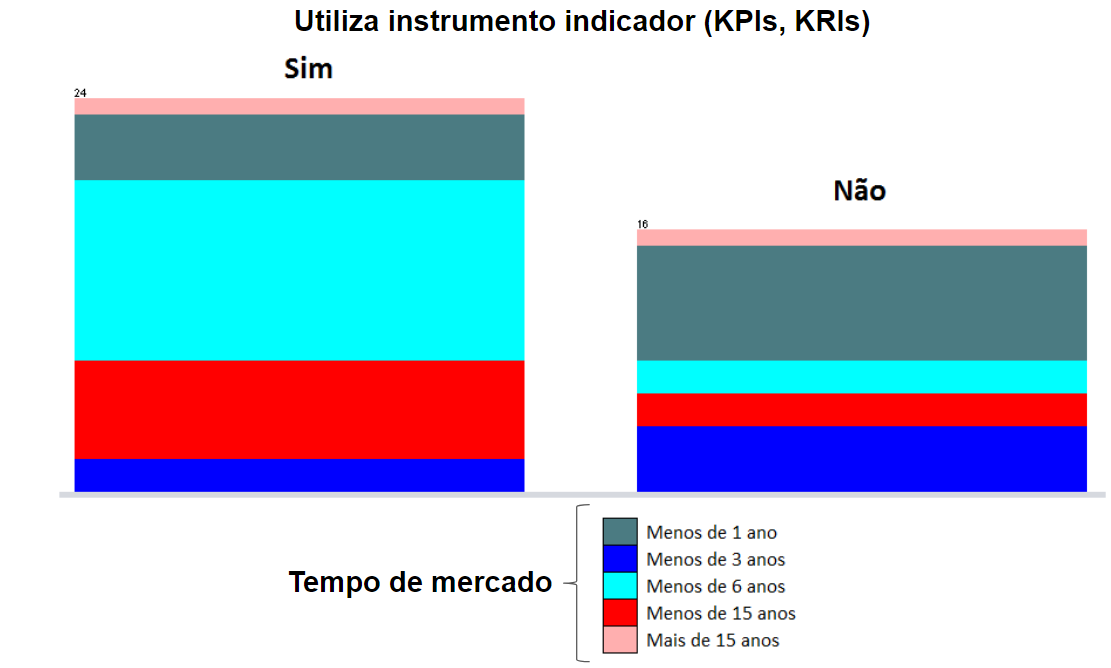
\includegraphics[width=13cm]{./fig/grafico05}
\caption{Utiliza instrumento indicador (KPIs, KRIs) X Tempo de mercado. (Fonte: Autoria própria, 2019)}
\label{fig:grafico49}
\end{figure}

As pessoas que informaram possuir nível de conhecimento em tecnologia da informação “Superior” utilizam algum instrumento indicador (KPIs, KRIs) em sua empresa, como demonstrado na figura \ref{fig:grafico411}. Todos os entrevistados que possuem nível de conhecimento em TI “mínimo” não utilizam instrumento indicador (KPIs, KRIs) em suas empresas.

% Imagem fixa
\begin{figure}[H]

\centering
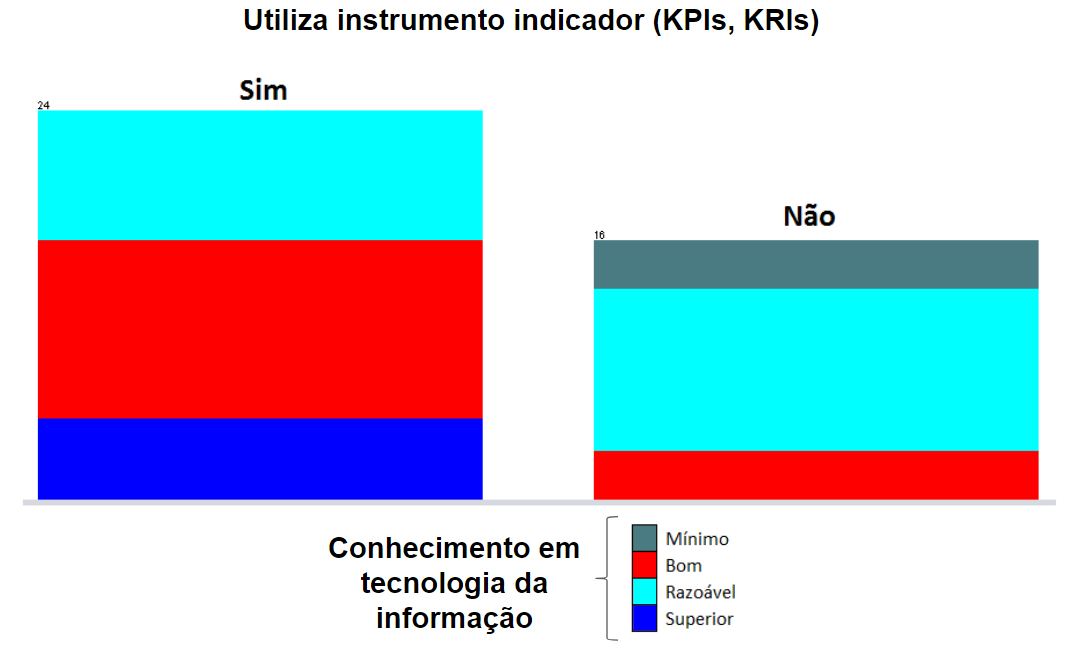
\includegraphics[width=13cm]{./fig/grafico08}
\caption{Utiliza instrumento indicador (KPIs, KRIs) X Conhecimento em TI. (Fonte: Autoria própria, 2019)}
\label{fig:grafico411}
\end{figure}

As pessoas com nível de conhecimento em TI “Superior” estão presentes no grupo que cria conteúdo relevante e o distribui em redes sociais e campanhas de e-mail marketing, como descrito na figura \ref{fig:grafico412}. Por outro lado, a maioria das pessoas com nível de conhecimento em TI “mínimo” não cria conteúdo relevante e o distribui em redes sociais e campanhas de e-mail marketing. 

% Imagem fixa
\begin{figure}[H]

\centering
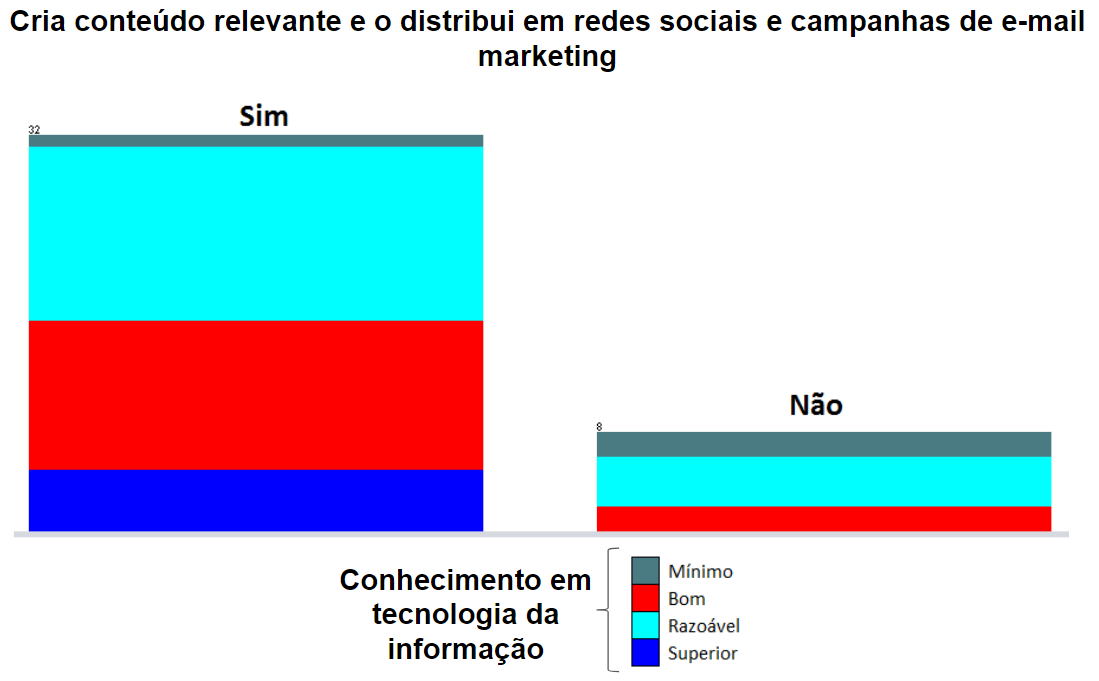
\includegraphics[width=13cm]{./fig/grafico09}
\caption{Cria conteúdo relevante e o distribui em redes sociais e campanhas de e-mail marketing X Conhecimento em TI. (Fonte: Autoria própria, 2019)}
\label{fig:grafico412}
\end{figure}

Na figura \ref{fig:grafico410} é mostrado que as empresas com maior tempo de mercado, em sua maioria, fazem o acompanhamento durante o período de pós-venda, monitorando o feedback dos clientes na internet, tanto em redes sociais como sites de reclamação, para poder melhorar um produto/serviço. Já as empresas com menos de 1 ano de atuação não fazem esse acompanhamento.

% Imagem fixa
\begin{figure}[H]

\centering
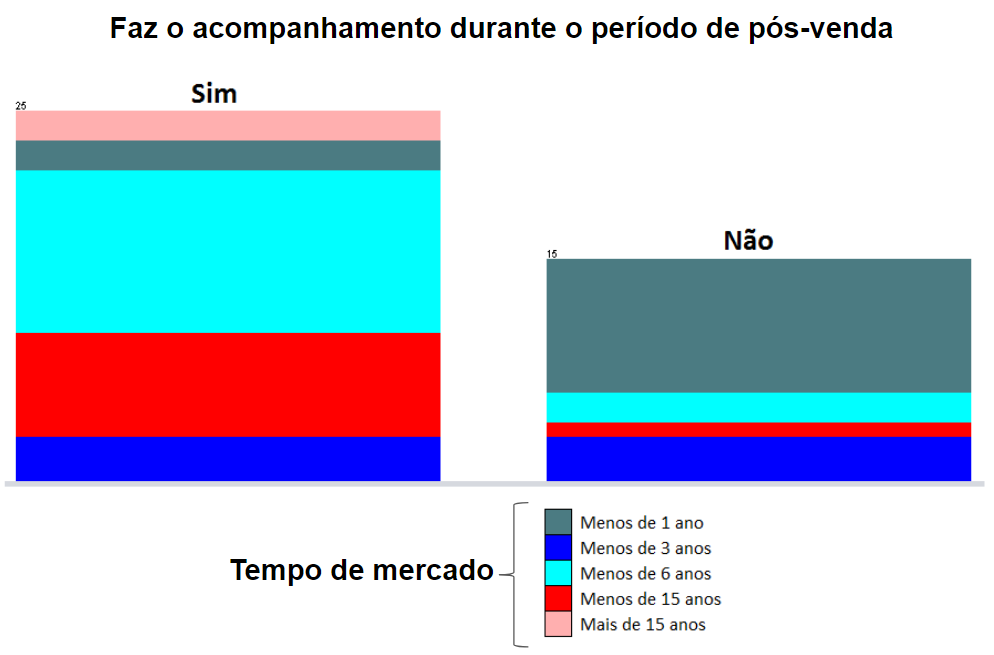
\includegraphics[width=13cm]{./fig/grafico06}
\caption{Faz o acompanhamento durante o período de pós-venda X Tempo de mercado. (Fonte: Autoria própria, 2019)}
\label{fig:grafico410}
\end{figure}

Na figura \ref{fig:grafico413} podemos ver a comparação das variáveis  “empresas que terceirizam alguma função específica, recurso ou infraestrutura de TI”, representado pelas duas colunas e “empresas que realizam a análise ambiental e promovem estudos de redesenho dos processos” representado pelas cores azul e vermelho. A pesquisa mostrou que a maioria das empresas que terceirizam alguma função específica, recurso ou infraestrutura de TI, realizam a análise ambiental e promovem estudos de redesenho dos processos. 

% Imagem fixa
\begin{figure}[H]

\centering
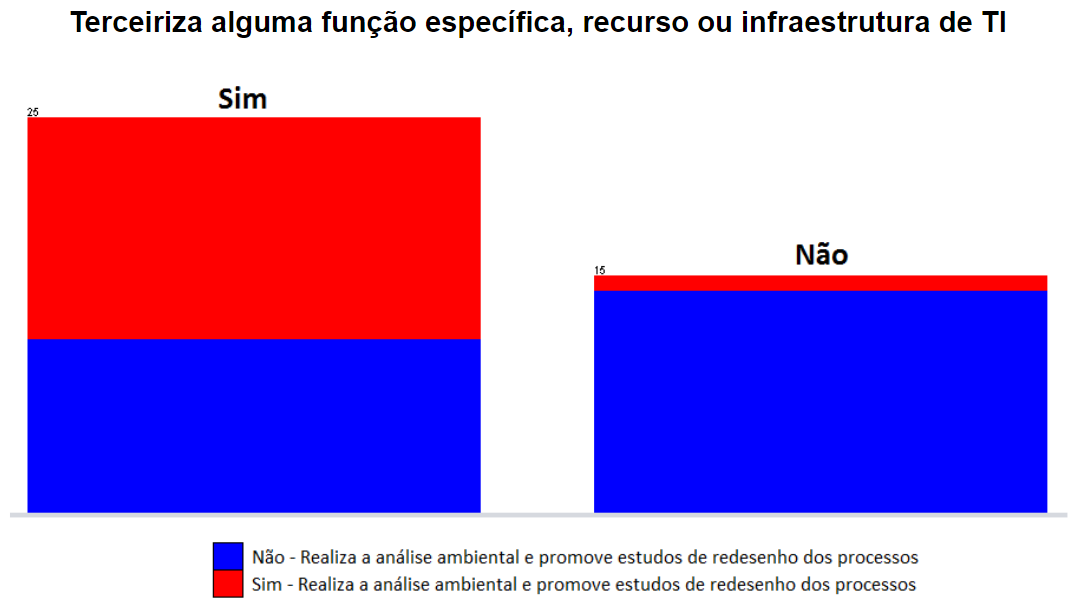
\includegraphics[width=13cm]{./fig/grafico11}
\caption{Terceirização e estudos de redesenho dos processos. (Fonte: Autoria própria, 2019)}
\label{fig:grafico413}
\end{figure}
	
Conforme a figura \ref{fig:grafico414}, foi identificado que as empresas que realizam a análise ambiental e promovem estudos de redesenho dos processos também utilizam, em sua totalidade, algum instrumento (indicador)  que monitora e acompanha o nível de desempenho (KPIs, satisfatório ou insatisfatório) e o nível de atingimento dos objetivos organizacionais (KRIs).

% Imagem fixa
\begin{figure}[H]

\centering
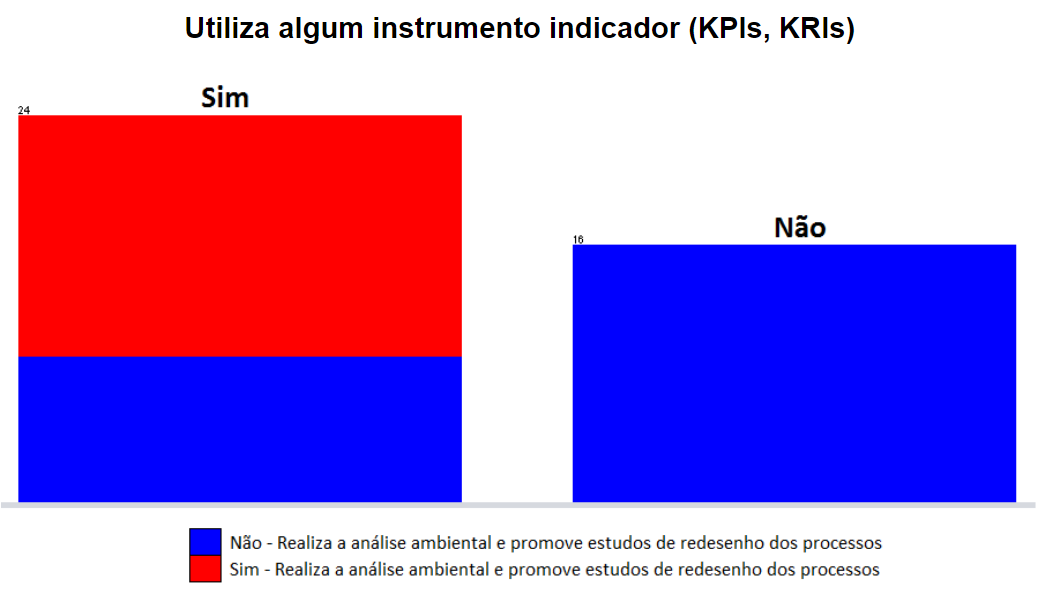
\includegraphics[width=13cm]{./fig/grafico12}
\caption{Utiliza algum instrumento indicador (KPIs, KRIs) X Promove redesenho dos processos. (Fonte: Autoria própria, 2019)}
\label{fig:grafico414}
\end{figure}


\section{Discussão dos resultados}
\label{subsec:framing}

Através dos dados, observa-se que as pessoas que possuem nível de conhecimento em tecnologia da informação “Bom” ou “Superior”, estão, em sua em sua maioria em empresas que possuem maior tempo de atuação no mercado, o que evidencia que o fator habilitador “conhecimento em tecnologia da informação”, citado na seção \ref{subsec:conhecimentoti}, exerce influência nas empresas que atuam de forma eletrônica.

As empresas que utilizam algum instrumento indicador que monitora e acompanha o nível de desempenho (KPIs, satisfatório, ou insatisfatório) e o nível de atingimento dos objetivos organizacionais (KRIs) são as que possuem maior tempo de atuação no mercado. Essa informação reforça a tese de que o fator habilitador “indicador de desempenho”, citado na seção \ref{subsec:kpi} deste estudo, contribui para um resultado satisfatório da organização. Efetuar a gestão da empresa utilizando indicador de desempenho (KPIs, KRIs) será um diferencial competitivo, e um fator crucial para a sobrevivência e crescimento no cenário em que a concorrência está cada vez maior e os clientes mais exigentes.

As pessoas que informaram possuir nível de conhecimento em tecnologia da informação “Superior” utilizam algum instrumento indicador (KPIs, KRIs) em sua empresa, essas pessoas também estão presentes no grupo que cria conteúdo relevante e o distribui em redes sociais e campanhas de e-mail marketing. O que mostra que, quanto maior o conhecimento em TI, presente nos empresários/gestores, mais habilitado estará essa organização para tomar decisões, seja para utilizar novas ferramentas ou manipular as que já existam na organização.

De acordo com a pesquisa, a maioria das empresas com menos de 1 ano de atuação não fazem o acompanhamento durante o período de pós-venda, monitorando o feedback dos clientes na internet, tanto em redes sociais como sites de reclamação, para poder melhorar um produto/serviço, como dito pelo Sebrae, na seção \ref{sec:vidautil}, que as empresas são iniciadas com falta de planejamento e deficiências de gestão. 

A maioria das empresas com mais de 3 anos de atuação no mercado faz o acompanhamento durante o período de pós-venda, monitorando o feedback dos clientes na internet, tanto em redes sociais como sites de reclamação, para poder melhorar um produto/serviço. Desta forma, é evidenciado que o fator habilitador “melhoria contínua”, seção \ref{subsec:bpr}, pode influenciar de forma positiva uma organização.

As empresas que realizam a análise ambiental promovendo estudos de redesenho dos processos, em sua maioria, são as que terceirizam alguma função específica, recurso ou infraestrutura de TI, descrito na seção \ref{subsec:terceirizacao}. O que mostra que as empresas que possuem o fator “melhoria contínua”, citado na seção \ref{subsec:bpr}, optam por terceirizar alguma função/recurso e assim se dedicar a outras atividades chave. A terceirização pode melhorar o desempenho das empresas que não têm conhecimentos ou não querem gastar seus recursos internos em certas áreas.


\chapter{Conclusão}
\label{cap:conclusion}

Este trabalho teve como objetivo principal identificar quais são os fatores habilitadores candidatos para definição de um modelo de negócio eletrônico para empreendimentos de pequeno e médio porte que atuam no segmento de tecnologia da informação. Inicialmente efetuou-se uma revisão da literatura sobre os empreendimentos de pequeno e médio porte - PME, a definição sobre os negócios digitais, o modelo de negócio segundo a abordagem de Alexander Osterwalder,  partindo-se posteriormente para a etapa de coleta de dados fundamentada primordialmente na pesquisa com uso de questionários. 

A revisão da literatura mostrou que não há uma definição amplamente aceita sobre as PMEs no Brasil e a literatura continua com dificuldades em defini-las. Ainda assim, o princípio fundamental das definições circula em torno do conceito utilizado pelo Sebrae e da legislação específica do país, que é utilizada pela Receita Federal e está na Lei Geral para Micro e Pequenas Empresas. 

O número de empresas que divulga/comercializa produtos/serviços online é cada vez maior, mostrando que é uma oportunidade de negócio dinâmica e interessante, mas isso não quer dizer que seja simples manter um negócio online. O tempo de vida útil das empresas que comercializam seus produtos online é bem menor se comparado às empresas físicas. Desta forma, ganham cada vez mais relevância as discussões sobre as condições que levam a esse resultado, no sentido de garantir que não venham a acontecer com tanta frequência. 

O trabalho realizado ao longo deste estudo permitiu alargar os conhecimentos teóricos relacionadas aos fatores que exercem influência em uma empresa, sejam eles fatores específicos, externos e internos. Os fatores externos à empresa apresentam variáveis situacionais que podem facilitar ou inibir o empreendedorismo na inicialização e durante o ciclo de vida da PME. Fatores externos macroambientais não são controláveis e o sucesso da PME geralmente depende da capacidade do empresário de lidar com eles. O ambiente interno inclui todos os fatores específicos da empresa que são influenciados por ações específicas praticados por ela, incluindo a disponibilidade de recursos e habilidades pessoais para exercer funções empresariais e o uso efetivo de recursos dentro da empresa.

Os fatores habilitadores estão ligados às características específicas de cada negócio. Em contrapartida, existem autores que não estudam aspectos do negócio em si, mas sim traços de personalidade do dirigente do empreendimento ou seus hábitos e práticas que podem levar ao sucesso do negócio. Como por exemplo a orientação empreendedora do dirigente da empresa que será composta por algumas características que influenciam positivamente o sucesso do empreendimento, dentre elas, a adaptação à mudança, iniciativa, propensão a assumir riscos e capacidade de aprender.

A revisão bibliográfica identificou alguns fatores habilitadores, dentre eles, o conhecimento de tecnologia da informação por parte dos empresários/gestores; a terceirização de funções específicas, recursos ou infraestruturas de TI; o uso dos marketplaces; o gerenciamento do estoque com a utilização do método cross docking; atuar em um mercado de nicho, segmentado; utilizar instrumento indicador que monitora e acompanha o nível de desempenho (KPIs, satisfatório, ou insatisfatório) e o nível de atingimento dos objetivos organizacionais (KRIs) e por fim, realizar a análise ambiental e promover estudos de redesenho, para garantir assim a melhoria contínua dos processos da empresa. A atuação de cada influenciador vai depender do ramo de atividade da empresa, uma vez que cada negócio possui suas características específicas. 

O estudo mostrou que alguns fatores habilitadores identificados estão presentes em parte das empresas que participaram da pesquisa. Como por exemplo, as empresas com gestores que possuem  nível de conhecimento em tecnologia da informação “Bom” ou “Superior”, ou que utilizam algum instrumento indicador que monitora e acompanha o nível de desempenho (KPIs, satisfatório, ou insatisfatório) e o nível de atingimento dos objetivos organizacionais (KRIs), estão, em sua em sua maioria, em empresas que possuem maior tempo de mercado. As pessoas que informaram possuir nível de conhecimento em tecnologia da informação “Superior” utilizam algum instrumento indicador (KPIs, KRIs) em sua empresa e as organizações com maior tempo de mercado, em sua maioria, fazem o acompanhamento durante o período de pós-venda, monitorando o feedback dos clientes na internet.

Este trabalho contribui com a comunidade acadêmica ao estudar os fatores habilitadores candidatos para definição de um modelo de negócio eletrônico para empreendimentos de pequeno e médio porte que atuam no segmento de tecnologia da informação. Ou seja, buscou-se destacar a importância dos fatores relacionados ao sucesso, ainda que de forma parcial. Além disso, este trabalho contribui ao meio acadêmico pela abordagem utilizada, uma vez que a pesquisa buscou obter a visão dos proprietários em detrimento da experiência dos usuários, essa mais frequentemente utilizada na avaliação da atuação das empresas.


\section{Limitações}
\label{sec:model}

Uma das limitações da pesquisa utilizada é inerente ao uso dos questionários como estratégia de pesquisa. Trata-se da baixa representatividade de empresas estudadas frente ao todo. Ou seja, o estudo de 55 casos, e casos estes somente brasileiros, apresenta-se como uma deficiência do trabalho.

\section{Trabalhos futuros}
\label{sec:model}

Na sequência do presente trabalho surgiram alguns aspectos que se revelaram interessantes para uma abordagem mais detalhada. De seguida, são referidos sumáriamente aqueles que poderão vir a ser objeto de futura investigação:
\begin{itemize}
\item Para trabalhos futuros seria interessante identificar como surgem e como se formam novos modelos de negócios nos diferentes setores da economia. 
\item Poderá desenvolver este trabalho numa perspetiva mais abrangente, selecionando para tal, uma amostra estatisticamente significativa, que poderia abranger PMEs que atuam de forma eletrônica em uma região geográfica maior.
\end{itemize}

%\input{./tex/cap_VI}

%------------------------------------------------------------ BIBLIOGRAFIA %
\cleardoublepage
%\nocite{*} %%% Retire esta linha para gerar a bibliografia com apenas as
           %%% referências usadas no seu texto!
\arial
\bibliographystyle{unsrt}
\bibliography{./bib/monografia} %%% Nomes dos seus arquivos .bib
\label{ref-bib}

%--------------------------------------------------------------- APÊNDICES %
\apendices
\chapter{Cronograma}
\label{apend:1}

% ######## init table ########
\begin{table}[h]
 \centering
 \caption{Cronograma}
% distancia entre a linha e o texto
 {\renewcommand\arraystretch{1.25}
 \begin{tabular}{ l l l l l l l l l l l l l l l l l l }
  \cline{1-1}\cline{2-2}\cline{3-3}\cline{4-4}\cline{5-5}\cline{6-6}\cline{7-7}\cline{8-8}\cline{9-9}\cline{10-10}\cline{11-11}\cline{12-12}\cline{13-13}\cline{14-14}\cline{15-15}\cline{16-16}\cline{17-17}\cline{18-18}  
    \multicolumn{1}{|c|}{  \centering } &
    \multicolumn{5}{c|}{2018 \centering } &
    \multicolumn{12}{c|}{2019 \centering }
  \\  
  \cline{1-1}\cline{2-2}\cline{3-3}\cline{4-4}\cline{5-5}\cline{6-6}\cline{7-7}\cline{8-8}\cline{9-9}\cline{10-10}\cline{11-11}\cline{12-12}\cline{13-13}\cline{14-14}\cline{15-15}\cline{16-16}\cline{17-17}\cline{18-18}  
    \multicolumn{1}{|c|}{ATIVIDADES} &
    \multicolumn{1}{c|}{a \centering } &
    \multicolumn{1}{c|}{s \centering } &
    \multicolumn{1}{c|}{o \centering } &
    \multicolumn{1}{c|}{n \centering } &
    \multicolumn{1}{c|}{d \centering } &
    \multicolumn{1}{c|}{j \centering } &
    \multicolumn{1}{c|}{f \centering } &
    \multicolumn{1}{c|}{m \centering } &
    \multicolumn{1}{c|}{a \centering } &
    \multicolumn{1}{c|}{m \centering } &
    \multicolumn{1}{c|}{j \centering } &
    \multicolumn{1}{c|}{j \centering } &
    \multicolumn{1}{c|}{a \centering } &
    \multicolumn{1}{c|}{s \centering } &
    \multicolumn{1}{c|}{o \centering } &
    \multicolumn{1}{c|}{n \centering } &
    \multicolumn{1}{c|}{d \centering }
  \\  
  \cline{1-1}\cline{2-2}\cline{3-3}\cline{4-4}\cline{5-5}\cline{6-6}\cline{7-7}\cline{8-8}\cline{9-9}\cline{10-10}\cline{11-11}\cline{12-12}\cline{13-13}\cline{14-14}\cline{15-15}\cline{16-16}\cline{17-17}\cline{18-18}  
    \multicolumn{1}{|c|}{Levantamento bibliográfico} &
    \multicolumn{1}{c|}{x} &
    \multicolumn{1}{c|}{x} &
    \multicolumn{1}{c|}{x} &
    \multicolumn{1}{c|}{x} &
    \multicolumn{1}{c|}{x} &
    \multicolumn{1}{c|}{x} &
    \multicolumn{1}{c|}{x} &
    \multicolumn{1}{c|}{x} &
    \multicolumn{1}{c|}{x} &
    \multicolumn{1}{c|}{x} &
    \multicolumn{1}{c|}{x} &
    \multicolumn{1}{c|}{x} &
    \multicolumn{1}{c|}{x} &
    \multicolumn{1}{c|}{x} &
    \multicolumn{1}{c|}{ } &
    \multicolumn{1}{c|}{ } &
    \multicolumn{1}{c|}{ }
  \\  
  \cline{1-1}\cline{2-2}\cline{3-3}\cline{4-4}\cline{5-5}\cline{6-6}\cline{7-7}\cline{8-8}\cline{9-9}\cline{10-10}\cline{11-11}\cline{12-12}\cline{13-13}\cline{14-14}\cline{15-15}\cline{16-16}\cline{17-17}\cline{18-18}  
    \multicolumn{1}{|c|}{Fichamentos} &
    \multicolumn{1}{c|}{ } &
    \multicolumn{1}{c|}{ } &
    \multicolumn{1}{c|}{ } &
    \multicolumn{1}{c|}{x} &
    \multicolumn{1}{c|}{x} &
    \multicolumn{1}{c|}{ } &
    \multicolumn{1}{c|}{ } &
    \multicolumn{1}{c|}{ } &
    \multicolumn{1}{c|}{ } &
    \multicolumn{1}{c|}{ } &
    \multicolumn{1}{c|}{ } &
    \multicolumn{1}{c|}{ } &
    \multicolumn{1}{c|}{ } &
    \multicolumn{1}{c|}{ } &
    \multicolumn{1}{c|}{ } &
    \multicolumn{1}{c|}{ } &
    \multicolumn{1}{c|}{ }
  \\  
  \cline{1-1}\cline{2-2}\cline{3-3}\cline{4-4}\cline{5-5}\cline{6-6}\cline{7-7}\cline{8-8}\cline{9-9}\cline{10-10}\cline{11-11}\cline{12-12}\cline{13-13}\cline{14-14}\cline{15-15}\cline{16-16}\cline{17-17}\cline{18-18}  
    \multicolumn{1}{|c|}{Pré projeto} &
    \multicolumn{1}{c|}{ } &
    \multicolumn{1}{c|}{ } &
    \multicolumn{1}{c|}{ } &
    \multicolumn{1}{c|}{ } &
    \multicolumn{1}{c|}{x} &
    \multicolumn{1}{c|}{x} &
    \multicolumn{1}{c|}{x} &
    \multicolumn{1}{c|}{x} &
    \multicolumn{1}{c|}{ } &
    \multicolumn{1}{c|}{ } &
    \multicolumn{1}{c|}{ } &
    \multicolumn{1}{c|}{ } &
    \multicolumn{1}{c|}{ } &
    \multicolumn{1}{c|}{ } &
    \multicolumn{1}{c|}{ } &
    \multicolumn{1}{c|}{ } &
    \multicolumn{1}{c|}{ }
  \\  
  \cline{1-1}\cline{2-2}\cline{3-3}\cline{4-4}\cline{5-5}\cline{6-6}\cline{7-7}\cline{8-8}\cline{9-9}\cline{10-10}\cline{11-11}\cline{12-12}\cline{13-13}\cline{14-14}\cline{15-15}\cline{16-16}\cline{17-17}\cline{18-18}  
    \multicolumn{1}{|c|}{Fatores candidatos} &
    \multicolumn{1}{c|}{ } &
    \multicolumn{1}{c|}{ } &
    \multicolumn{1}{c|}{ } &
    \multicolumn{1}{c|}{ } &
    \multicolumn{1}{c|}{ } &
    \multicolumn{1}{c|}{ } &
    \multicolumn{1}{c|}{ } &
    \multicolumn{1}{c|}{x} &
    \multicolumn{1}{c|}{x} &
    \multicolumn{1}{c|}{x} &
    \multicolumn{1}{c|}{x} &
    \multicolumn{1}{c|}{x} &
    \multicolumn{1}{c|}{x} &
    \multicolumn{1}{c|}{ } &
    \multicolumn{1}{c|}{ } &
    \multicolumn{1}{c|}{ } &
    \multicolumn{1}{c|}{ }
  \\  
  \cline{1-1}\cline{2-2}\cline{3-3}\cline{4-4}\cline{5-5}\cline{6-6}\cline{7-7}\cline{8-8}\cline{9-9}\cline{10-10}\cline{11-11}\cline{12-12}\cline{13-13}\cline{14-14}\cline{15-15}\cline{16-16}\cline{17-17}\cline{18-18}  
    \multicolumn{1}{|c|}{Redação monografia} &
    \multicolumn{1}{c|}{ } &
    \multicolumn{1}{c|}{ } &
    \multicolumn{1}{c|}{ } &
    \multicolumn{1}{c|}{ } &
    \multicolumn{1}{c|}{ } &
    \multicolumn{1}{c|}{ } &
    \multicolumn{1}{c|}{ } &
    \multicolumn{1}{c|}{ } &
    \multicolumn{1}{c|}{x} &
    \multicolumn{1}{c|}{x} &
    \multicolumn{1}{c|}{x} &
    \multicolumn{1}{c|}{x} &
    \multicolumn{1}{c|}{x} &
    \multicolumn{1}{c|}{x} &
    \multicolumn{1}{c|}{x} &
    \multicolumn{1}{c|}{x} &
    \multicolumn{1}{c|}{ }
  \\  
  \cline{1-1}\cline{2-2}\cline{3-3}\cline{4-4}\cline{5-5}\cline{6-6}\cline{7-7}\cline{8-8}\cline{9-9}\cline{10-10}\cline{11-11}\cline{12-12}\cline{13-13}\cline{14-14}\cline{15-15}\cline{16-16}\cline{17-17}\cline{18-18}  
    \multicolumn{1}{|c|}{Aplicação questionário} &
    \multicolumn{1}{c|}{ } &
    \multicolumn{1}{c|}{ } &
    \multicolumn{1}{c|}{ } &
    \multicolumn{1}{c|}{ } &
    \multicolumn{1}{c|}{ } &
    \multicolumn{1}{c|}{ } &
    \multicolumn{1}{c|}{ } &
    \multicolumn{1}{c|}{ } &
    \multicolumn{1}{c|}{ } &
    \multicolumn{1}{c|}{ } &
    \multicolumn{1}{c|}{ } &
    \multicolumn{1}{c|}{ } &
    \multicolumn{1}{c|}{ } &
    \multicolumn{1}{c|}{ } &
    \multicolumn{1}{c|}{x} &
    \multicolumn{1}{c|}{x} &
    \multicolumn{1}{c|}{ }
  \\  
  \cline{1-1}\cline{2-2}\cline{3-3}\cline{4-4}\cline{5-5}\cline{6-6}\cline{7-7}\cline{8-8}\cline{9-9}\cline{10-10}\cline{11-11}\cline{12-12}\cline{13-13}\cline{14-14}\cline{15-15}\cline{16-16}\cline{17-17}\cline{18-18}  
    \multicolumn{1}{|c|}{Análise dos resultados} &
    \multicolumn{1}{c|}{ } &
    \multicolumn{1}{c|}{ } &
    \multicolumn{1}{c|}{ } &
    \multicolumn{1}{c|}{ } &
    \multicolumn{1}{c|}{ } &
    \multicolumn{1}{c|}{ } &
    \multicolumn{1}{c|}{ } &
    \multicolumn{1}{c|}{ } &
    \multicolumn{1}{c|}{ } &
    \multicolumn{1}{c|}{ } &
    \multicolumn{1}{c|}{ } &
    \multicolumn{1}{c|}{ } &
    \multicolumn{1}{c|}{ } &
    \multicolumn{1}{c|}{ } &
    \multicolumn{1}{c|}{ } &
    \multicolumn{1}{c|}{x} &
    \multicolumn{1}{c|}{ }
  \\  
  \cline{1-1}\cline{2-2}\cline{3-3}\cline{4-4}\cline{5-5}\cline{6-6}\cline{7-7}\cline{8-8}\cline{9-9}\cline{10-10}\cline{11-11}\cline{12-12}\cline{13-13}\cline{14-14}\cline{15-15}\cline{16-16}\cline{17-17}\cline{18-18}  
    \multicolumn{1}{|c|}{Defesa} &
    \multicolumn{1}{c|}{ } &
    \multicolumn{1}{c|}{ } &
    \multicolumn{1}{c|}{ } &
    \multicolumn{1}{c|}{ } &
    \multicolumn{1}{c|}{ } &
    \multicolumn{1}{c|}{ } &
    \multicolumn{1}{c|}{ } &
    \multicolumn{1}{c|}{ } &
    \multicolumn{1}{c|}{ } &
    \multicolumn{1}{c|}{ } &
    \multicolumn{1}{c|}{ } &
    \multicolumn{1}{c|}{ } &
    \multicolumn{1}{c|}{ } &
    \multicolumn{1}{c|}{ } &
    \multicolumn{1}{c|}{ } &
    \multicolumn{1}{c|}{ } &
    \multicolumn{1}{c|}{x}
  \\  
  \cline{1-1}\cline{2-2}\cline{3-3}\cline{4-4}\cline{5-5}\cline{6-6}\cline{7-7}\cline{8-8}\cline{9-9}\cline{10-10}\cline{11-11}\cline{12-12}\cline{13-13}\cline{14-14}\cline{15-15}\cline{16-16}\cline{17-17}\cline{18-18}  
    \multicolumn{1}{|c|}{Divulgação} &
    \multicolumn{1}{c|}{ } &
    \multicolumn{1}{c|}{ } &
    \multicolumn{1}{c|}{ } &
    \multicolumn{1}{c|}{ } &
    \multicolumn{1}{c|}{ } &
    \multicolumn{1}{c|}{ } &
    \multicolumn{1}{c|}{ } &
    \multicolumn{1}{c|}{ } &
    \multicolumn{1}{c|}{ } &
    \multicolumn{1}{c|}{ } &
    \multicolumn{1}{c|}{ } &
    \multicolumn{1}{c|}{ } &
    \multicolumn{1}{c|}{ } &
    \multicolumn{1}{c|}{ } &
    \multicolumn{1}{c|}{ } &
    \multicolumn{1}{c|}{ } &
    \multicolumn{1}{c|}{x}
  \\  
  \hline

 \end{tabular} }
\end{table}


\textbf{Ordem cronológica dos meses: }a = agosto, s = setembro, o = outubro, n = novembro, d = dezembro, j = janeiro, f = fevereiro, m = março, a = abril, m = maio, j = junho, j = julho, a = agosto, s = setembro, o = outubro, n = novembro, d = dezembro. 
\chapter{Questionário}
\label{apend:2}

Caro empresário/gestor, estou realizando um estudo que pretende identificar fatores habilitadores para definição de um modelo de negócio eletrônico para empresas do arranjo produtivo local. O questionário visa identificar o quanto sua empresa está aderente a esses fatores. Para o êxito desta pesquisa é essencial que o questionário seja respondido na íntegra, até o dia 07 de novembro de 2019. Será mantida a confidencialidade com respeito a todas as informações fornecidas.

O número de empresas que divulga/comercializa produtos/serviços online é cada vez maior, mostrando que é uma oportunidade de negócio dinâmica e interessante, mas isso não quer dizer que seja simples manter um negócio online. Pesquisas mostram que o tempo de vida útil das empresas que comercializam seus produtos online é bem menor se comparado às empresas físicas.

Há inúmeros fatores considerados habilitadores para definição de um modelo de negócio eletrônico, a começar pelo posicionamento estratégico. Em geral, os fatores candidatos a potencializar o negócio no ambiente eletrônico estão presentes em áreas específicas da empresa, em práticas e processos, ou em funções de negócio, considerados como chaves para o sucesso de uma organização.

Esta pesquisa faz parte do Trabalho Final de Curso do Bacharelado em Sistemas de Informação (Instituto de Informática da Universidade Federal de Goiás). Todas as informações coletadas servirão única e exclusivamente para subsidiar as análises do trabalho acadêmico. Portanto, será mantida a confidencialidade e a divulgação ficará restrita aos grandes números (agregados), ou seja, sem a necessidade de vincular à sua empresa.

Ao final da pesquisa, o resultado será disponibilizado a todos que responderem este questionário.

\begin{table}[]
\begin{tabular}{l}
Orlando da Cruz Pereira Júnior \\
Graduando em Sistemas de Informação - INF/UFG \\
Orientador: Prof. Dr. Eliomar Araújo de Lima \\
Telefone: (62) 98478-1195 \\
E-mail: orlando\_junior@discente.ufg.br
\end{tabular}
\end{table}

%========================================================================
% Perguntas do questionário

\begin{table}[]
\begin{tabular}{l}
\textbf{SEÇÃO 1} \\
\\
1- Nome (Opcional) \\
\_\_\_\_\_\_\_\_\_\_\_\_\_\_\_\_\_\_\_\_\_\_\_\_\_\_\_\_\_\_\_\_\_\_\_\_\_\_\_\_\_\_\_\_\_\_\_\_\_\_ \\
\\
2- E-mail \\
\_\_\_\_\_\_\_\_\_\_\_\_\_\_\_\_\_\_\_\_\_\_\_\_\_\_\_\_\_\_\_\_\_\_\_\_\_\_\_\_\_\_\_\_\_\_\_\_\_\_ \\
\\
3- Empresa (Opcional) \\
\_\_\_\_\_\_\_\_\_\_\_\_\_\_\_\_\_\_\_\_\_\_\_\_\_\_\_\_\_\_\_\_\_\_\_\_\_\_\_\_\_\_\_\_\_\_\_\_\_\_ \\
\\
4- Cargo que ocupa na empresa \\
\_\_\_\_\_\_\_\_\_\_\_\_\_\_\_\_\_\_\_\_\_\_\_\_\_\_\_\_\_\_\_\_\_\_\_\_\_\_\_\_\_\_\_\_\_\_\_\_\_\_ \\
\\
5- Celular ou telefone de contato (Opcional) \\
\_\_\_\_\_\_\_\_\_\_\_\_\_\_\_\_\_\_\_\_\_\_\_\_\_\_\_\_\_\_\_\_\_\_\_\_\_\_\_\_\_\_\_\_\_\_\_\_\_\_ \\
\\
\begin{tabular}[c]{@{}l@{}}6- A empresa comercializa seus produtos/serviços em canais\\ eletrônicos (e-commerce)?\end{tabular} \\
(   ) Sim - Prossiga na seção 2, da pergunta 7 a 19. \\
(   ) Não - Prossiga na seção 3, da pergunta 7 a 16.
\end{tabular}
\end{table}

%=========================================================================
% Seção 2

\begin{table}[]
\begin{tabular}{l}
\textbf{SEÇÃO 2 - Comercializa produtos/serviços em canais eletrônicos (e-commerce)} \\
 \\
7- Tipicação da Empresa/Organização? \\
(   ) PME \\
(   ) Grande porte \\
(   ) Startup \\
(   ) Fintech \\
(   ) Encubadora/Aceleradora \\
 \\
8- Tempo de mercado \\
(   ) Menos de 1 ano \\
(   ) Menos de 3 anos \\
(   ) Menos de 6 anos \\
(   ) Menos de 15 anos \\
(   ) Mais de 15 anos \\
 \\
9- Área de Atuação da Empresa \\
(   ) Desenvolvimento de soluções de ERP, SIG, BPM \\
(   ) Suporte Técnico e Infraestrutura de TI \\
(   ) Assessoria e consultoria em TI \\
(   ) Outsourcing (BPO, KPO, ...) \\
(   ) Desenvolvimento de soluções Fullstack \\
(   ) Desenvolvimento de soluções mobile \\
(   ) Desenvolvimento de soluções de CRM, BI \\
\begin{tabular}[c]{@{}l@{}}(   ) Desenvolvimento de soluções de Cloud, Big Data, Data Science, Machine Learning e\\ Deep Learning\end{tabular} \\
(   ) Certicadora/Homologadora \\
(   ) Capacitação e Qualicação prossional \\
(   ) Mentoring e/ou Coaching \\
(   ) Comércio de suprimentos de informática \\
(   ) Outro: \_\_\_\_\_\_\_\_\_\_\_\_\_\_\_\_\_\_\_\_\_\_\_\_\_\_ \\
 \\
\begin{tabular}[c]{@{}l@{}}10- Como você avalia seu nível de conhecimento em tecnologia da\\ informação?\end{tabular} \\
(   ) Mínimo \\
(   ) Razoável \\
(   ) Bom \\
(   ) Superior \\
 \\
\begin{tabular}[c]{@{}l@{}}11- A empresa terceiriza alguma função especíca, recurso ou\\ infraestrutura de TI?\end{tabular} \\
(   ) Sim \\
(   ) Não \\
\end{tabular}
\end{table}

%===============================

\begin{table}[]
\begin{tabular}{l}
\begin{tabular}[c]{@{}l@{}}12- Em quais plataformas a empresa divulga/comercializa\\ produtos/serviços on-line?\end{tabular} \\
(   ) Plataforma própria (Desenvolvida e mantida pela empresa) \\
(   ) Plataforma Terceirizada (Loja integrada, WIX, Tray, outros) \\
(   ) Redes sociais (Facebook, Instagram, outros) \\
(   ) Marketplace (Google Play Store, Mercado Livre, B2W, outros) \\
(   ) Outros. \\
 \\
\begin{tabular}[c]{@{}l@{}}13- Utiliza a modalidade Cross-docking na empresa, em que, por meio de\\ um acordo com fornecedores, a loja vende antes de comprar e\\ estabelece o prazo de entrega, considerando o tempo de reposição do\\ fornecedor?\end{tabular} \\
(   ) Sim \\
(   ) Não \\
 \\
\begin{tabular}[c]{@{}l@{}}14- A empresa mapeia o perfil de seu consumidor e atua em um\\ mercado de nicho, segmentado?\end{tabular} \\
(   ) Sim \\
(   ) Não \\
 \\
\begin{tabular}[c]{@{}l@{}}15- Realiza a análise ambiental e promove estudos de redesenho\\ (pivotar) dos processos da empresa regularmente?\end{tabular} \\
(   ) Sim \\
(   ) Não \\
 \\
\begin{tabular}[c]{@{}l@{}}16- A empresa utiliza algum instrumento (indicador) que monitora e\\ acompanha o nível de desempenho (KPIs, satisfatório ou insatisfatório)\\ e o nível de atingimento dos objetivos organizacionais (KRIs)?\end{tabular} \\
(   ) Sim \\
(   ) Não \\
 \\
\begin{tabular}[c]{@{}l@{}}17- A empresa faz parte de alguma comunidade empresarial, seja ela\\ cooperativa ou associativa?\end{tabular} \\
(   ) Sim \\
(   ) Não \\
 \\
\begin{tabular}[c]{@{}l@{}}18- A empresa atua na criação de conteúdo relevante para o seu público\\ alvo e o distribui por meio de blogs, redes sociais e campanhas de e-mail\\ marketing?\end{tabular} \\
(   ) Sim \\
(   ) Não \\
 \\
\begin{tabular}[c]{@{}l@{}}19- A empresa faz o acompanhamento durante o período de pós-venda,\\ monitorando o feedback dos clientes na internet, tanto em redes sociais\\ como em sites de reclamação, para poder melhorar um produto/serviço?\end{tabular} \\
(   ) Sim \\
(   ) Não
\end{tabular}
\end{table}

%=========================================================================
% Seção 3

\begin{table}[]
\begin{tabular}{l}
\textbf{SEÇÃO 3 - Não comercializa produtos/serviços on-line} \\
 \\
7- Tipicação da Empresa/Organização? \\
(   ) PME \\
(   ) Grande porte \\
(   ) Startup \\
(   ) Fintech \\
(   ) Encubadora/Aceleradora \\
 \\
8- Tempo de mercado \\
(   ) Menos de 1 ano \\
(   ) Menos de 3 anos \\
(   ) Menos de 6 anos \\
(   ) Menos de 15 anos \\
(   ) Mais de 15 anos \\
 \\
9- Área de Atuação da Empresa \\
(   ) Desenvolvimento de soluções de ERP, SIG, BPM \\
(   ) Suporte Técnico e Infraestrutura de TI \\
(   ) Assessoria e consultoria em TI \\
(   ) Outsourcing (BPO, KPO, ...) \\
(   ) Desenvolvimento de soluções Fullstack \\
(   ) Desenvolvimento de soluções mobile \\
(   ) Desenvolvimento de soluções de CRM, BI \\
\begin{tabular}[c]{@{}l@{}}(   ) Desenvolvimento de soluções de Cloud, Big Data, Data Science, Machine Learning e\\ Deep Learning\end{tabular} \\
(   ) Certicadora/Homologadora \\
(   ) Capacitação e Qualicação prossional \\
(   ) Mentoring e/ou Coaching \\
(   ) Comércio de suprimentos de informática \\
(   ) Outro: \_\_\_\_\_\_\_\_\_\_\_\_\_\_\_\_\_\_\_\_\_\_\_\_\_\_ \\
 \\
\begin{tabular}[c]{@{}l@{}}10- Como você avalia seu nível de conhecimento em tecnologia da\\ informação?\end{tabular} \\
(   ) Mínimo \\
(   ) Razoável \\
(   ) Bom \\
(   ) Superior \\
 \\
\begin{tabular}[c]{@{}l@{}}11- A empresa terceiriza alguma função especíca, recurso ou\\ infraestrutura de TI?\end{tabular} \\
(   ) Sim \\
(   ) Não \\
 \\
\end{tabular}
\end{table}

%===============================

\begin{table}[]
\begin{tabular}{l}
\begin{tabular}[c]{@{}l@{}}12- A empresa trabalha de forma que não precisa armazenar produtos
em estoque por \\muito tempo (just-in-time)? \end{tabular} \\
(   ) Sim \\
(   ) Não \\
 \\
\begin{tabular}[c]{@{}l@{}}13- A empresa mapeia o perfil de seu consumidor e atua em um\\ mercado de nicho, segmentado?\end{tabular} \\
(   ) Sim \\
(   ) Não \\
 \\
\begin{tabular}[c]{@{}l@{}}14- Realiza a análise ambiental e promove estudos de redesenho\\ (pivotar) dos processos da empresa regularmente?\end{tabular} \\
(   ) Sim \\
(   ) Não \\
 \\
\begin{tabular}[c]{@{}l@{}}15- A empresa utiliza algum instrumento (indicador) que monitora e\\ acompanha o nível de desempenho (KPIs, satisfatório ou insatisfatório)\\ e o nível de atingimento dos objetivos organizacionais (KRIs)?\end{tabular} \\
(   ) Sim \\
(   ) Não \\
 \\
\begin{tabular}[c]{@{}l@{}}16- A empresa faz parte de alguma comunidade empresarial, seja ela\\ cooperativa ou associativa?\end{tabular} \\
(   ) Sim \\
(   ) Não \\
\end{tabular}
\end{table}

\end{document}

%------------------------------------------------------------------------- %
%        F I M   D O  A R Q U I V O :  m o d e l o - t e s e . t e x       %
%------------------------------------------------------------------------- %
